\documentclass[a4paper, openany]{book}
%\documentclass{tuftebook}
\usepackage{graphicx}
\usepackage[export]{adjustbox}
\usepackage{amsthm}
\usepackage[many]{tcolorbox}
\usepackage[margin=0.75in]{geometry}
\usepackage{amsfonts}
\usepackage{mathtools}
\usepackage{enumerate}
\usepackage{wrapfig}
\usepackage[makeroom]{cancel}

\makeatletter

\makeatletter

\def\renewtheorem#1{%
	\expandafter\let\csname#1\endcsname\relax
	\expandafter\let\csname c@#1\endcsname\relax
	\gdef\renewtheorem@envname{#1}
	\renewtheorem@secpar
}
\def\renewtheorem@secpar{\@ifnextchar[{\renewtheorem@numberedlike}{\renewtheorem@nonumberedlike}}
\def\renewtheorem@numberedlike[#1]#2{\newtheorem{\renewtheorem@envname}[#1]{#2}}
\def\renewtheorem@nonumberedlike#1{
	\def\renewtheorem@caption{#1}
	\edef\renewtheorem@nowithin{\noexpand\newtheorem{\renewtheorem@envname}{\renewtheorem@caption}}
	\renewtheorem@thirdpar
}
\def\renewtheorem@thirdpar{\@ifnextchar[{\renewtheorem@within}{\renewtheorem@nowithin}}
\def\renewtheorem@within[#1]{\renewtheorem@nowithin[#1]}

\makeatother

%%%%%%%%%%%%%%%%%%%%
% New environments %
%%%%%%%%%%%%%%%%%%%%

\makeatother
%\mdfsetup{skipabove=1em,skipbelow=0em}

\tcbuselibrary{skins}

% Color definitions

\definecolor{proofcolor}{RGB}{0,0,0}

% Dark orange and Dark Red rgb
%\definecolor{theorembordercolor}{RGB}{151, 63, 5}
%\definecolor{theorembackgroundcolor}{RGB}{248, 241, 234}
\definecolor{theorembordercolor}{RGB}{255, 165, 0}
\definecolor{theorembackgroundcolor}{RGB}{254, 249, 243}

%\definecolor{examplebordercolor}{RGB}{0, 110, 184}
\definecolor{remarkbackgroundcolor}{RGB}{240, 244, 250}

\definecolor{examplebordercolor}{RGB}{199, 0, 57}
\definecolor{examplebackgroundcolor}{RGB}{248, 241, 234}

\definecolor{remarkbordercolor}{RGB}{0, 110, 184}

\definecolor{definitionbordercolor}{RGB}{0, 150, 85}
\definecolor{definitionbackgroundcolor}{RGB}{239, 247, 243}

\definecolor{propertybordercolor}{RGB}{128, 0, 128}
\definecolor{propertybackgroundcolor}{RGB}{255, 240, 255}

\definecolor{formulabordercolor}{RGB}{0, 0, 0}
\definecolor{formulabackgroundcolor}{RGB}{230, 229, 245}

\newtheoremstyle{theorem}
{0pt}{0pt}{\normalfont}{0pt}
{}{\;}{0.25em}
{{\sffamily\bfseries\color{theorembordercolor}\thmname{#1}~\thmnumber{\textup{#2}}.}
	\thmnote{\normalfont\color{black}~(#3)}}

\newtheoremstyle{definition}
{0pt}{0pt}{\normalfont}{0pt}
{}{\;}{0.25em}
{{\sffamily\bfseries\color{definitionbordercolor}\thmname{#1}~\thmnumber{\textup{#2}}.}
	\thmnote{\normalfont\color{black}~(#3)}}

\newtheoremstyle{notation}
{0pt}{0pt}{\normalfont}{0pt}
{}{\;}{0.25em}
{{\sffamily\bfseries\color{definitionbordercolor}\thmname{#1}~\thmnumber{\textup{#2}}.}
	\thmnote{\normalfont\color{black}~(#3)}}

\newtheoremstyle{example}
{0pt}{0pt}{\normalfont}{0pt}
{}{\;}{0.25em}
{{\sffamily\bfseries\color{examplebordercolor}\thmname{#1}~\thmnumber{\textup{#2}}.}
	\thmnote{\normalfont\color{black}~(#3)}}
	
\newtheoremstyle{remark}
{0pt}{0pt}{\normalfont}{0pt}
{}{\;}{0.25em}
{{\sffamily\bfseries\color{remarkbordercolor}\thmname{#1}.}
	\thmnote{\normalfont\color{black}~(#3)}}	

\newtheoremstyle{property}
{0pt}{0pt}{\normalfont}{0pt}
{}{\;}{0.25em}
{{\sffamily\bfseries\color{propertybordercolor}\thmname{#1}~\thmnumber{\textup{#2}}.}
	\thmnote{\normalfont\color{black}~(#3)}}

\newtheoremstyle{formula}
{0pt}{0pt}{\normalfont}{0pt}
{}{\;}{0.25em}
{{\sffamily\bfseries\color{formulabordercolor}\thmname{#1}~\thmnumber{\textup{#2}}.}
	\thmnote{\normalfont\color{black}~(#3)}}

%%%%%%%%%%%%%%%%%%%%%%%%
% Theorem Environments %
%%%%%%%%%%%%%%%%%%%%%%%%

\theoremstyle{theorem}

\newtheorem{theorem}{Theorem}
\newtheorem{contrapositive}{Contrapositive}
\numberwithin{theorem}{section}
\numberwithin{contrapositive}{section}
\newtheorem{postulate}{Postulate}
\newtheorem{conjecture}{Conjecture}
%\newtheorem{corollary}{Corollary}
%\newtheorem{lemma}{Lemma}
\newtheorem{conclusion}{Conclusion}

\tcolorboxenvironment{theorem}{
	enhanced jigsaw, pad at break*=1mm, breakable,
	left=4mm, right=4mm, top=1mm, bottom=1mm,
	colback=theorembackgroundcolor, boxrule=0pt, frame hidden,
	borderline west={0.5mm}{0mm}{theorembordercolor}, arc=.5mm
}
\tcolorboxenvironment{contrapositive}{
	enhanced jigsaw, pad at break*=1mm, breakable,
	left=4mm, right=4mm, top=1mm, bottom=1mm,
	colback=theorembackgroundcolor, boxrule=0pt, frame hidden,
	borderline west={0.5mm}{0mm}{theorembordercolor}, arc=.5mm
}
\tcolorboxenvironment{postulate}{
	enhanced jigsaw, pad at break*=1mm, breakable,
	left=4mm, right=4mm, top=1mm, bottom=1mm,
	colback=theorembackgroundcolor, boxrule=0pt, frame hidden,
	borderline west={0.5mm}{0mm}{theorembordercolor}, arc=.5mm
}
\tcolorboxenvironment{conjecture}{
	enhanced jigsaw, pad at break*=1mm, breakable,
	left=4mm, right=4mm, top=1mm, bottom=1mm,
	colback=theorembackgroundcolor, boxrule=0pt, frame hidden,
	borderline west={0.5mm}{0mm}{theorembordercolor}, arc=.5mm
}
%\tcolorboxenvironment{corollary}{
%	enhanced jigsaw, pad at break*=1mm, breakable,
%	left=4mm, right=4mm, top=1mm, bottom=1mm,
%	colback=theorembackgroundcolor, boxrule=0pt, frame hidden,
%	borderline west={0.5mm}{0mm}{theorembordercolor}, arc=.5mm
%}
%\tcolorboxenvironment{lemma}{
%	enhanced jigsaw, pad at break*=1mm, breakable,
%	left=4mm, right=4mm, top=1mm, bottom=1mm,
%	colback=theorembackgroundcolor, boxrule=0pt, frame hidden,
%	borderline west={0.5mm}{0mm}{theorembordercolor}, arc=.5mm
%}
\tcolorboxenvironment{conclusion}{
	enhanced jigsaw, pad at break*=1mm, breakable,
	left=4mm, right=4mm, top=1mm, bottom=1mm,
	colback=theorembackgroundcolor, boxrule=0pt, frame hidden,
	borderline west={0.5mm}{0mm}{theorembordercolor}, arc=.5mm
}

%%%%%%%%%%%%%%%%%%%%%%%%%%%
% Definition Environments %
%%%%%%%%%%%%%%%%%%%%%%%%%%%

\theoremstyle{definition}
\newtheorem{definition}{Definition}
\numberwithin{definition}{section}
\newtheorem{review}{Review}
\newtheorem*{notation}{Notation}
\tcolorboxenvironment{notation}{
	enhanced jigsaw, pad at break*=1mm, breakable,
	left=4mm, right=4mm, top=1mm, bottom=1mm,
	colback=white, boxrule=0pt, frame hidden,
	borderline west={0.5mm}{0mm}{definitionbordercolor},
	borderline east={0.5mm}{0mm}{definitionbordercolor},
	borderline north={0.5mm}{0mm}{definitionbordercolor},
	borderline south={0.5mm}{0mm}{definitionbordercolor},
	 arc=.5mm
}

\tcolorboxenvironment{definition}{
	enhanced jigsaw, pad at break*=1mm, breakable,
	left=4mm, right=4mm, top=1mm, bottom=1mm,
	colback=definitionbackgroundcolor, boxrule=0pt, frame hidden,
	borderline west={0.5mm}{0mm}{definitionbordercolor}, arc=.5mm
}
\tcolorboxenvironment{review}{
	enhanced jigsaw, pad at break*=1mm, breakable,
	left=4mm, right=4mm, top=1mm, bottom=1mm,
	colback=definitionbackgroundcolor, boxrule=0pt, frame hidden,
	borderline west={0.5mm}{0mm}{definitionbordercolor}, arc=.5mm
}


%%%%%%%%%%%%%%%%%%%%%%%%
% Example Environments %
%%%%%%%%%%%%%%%%%%%%%%%%

\theoremstyle{example}
\newtheorem{example}{Example}
\numberwithin{example}{section}
%\newtheorem*{remark}{Remark}
%\newtheorem*{note}{Note}

\tcolorboxenvironment{example}{
	enhanced jigsaw, pad at break*=1mm, breakable,
	left=4mm, right=4mm, top=1mm, bottom=1mm,
	colback=examplebackgroundcolor, boxrule=0pt, frame hidden,
	borderline west={0.5mm}{0mm}{examplebordercolor}, arc=.5mm
}

\theoremstyle{remark}
\newtheorem{remark}{Remark}
\newtheorem*{note}{Note}
\newtheorem*{recall}{Recall}
\newtheorem{observation}{Observation}
\newtheorem{fact}{Fact}
\tcolorboxenvironment{remark}{
	enhanced jigsaw, pad at break*=1mm, breakable,
	left=4mm, right=4mm, top=1mm, bottom=1mm,
	colback=white, boxrule=0pt, frame hidden,
	borderline west={0.5mm}{0mm}{remarkbordercolor},
	borderline east={0.5mm}{0mm}{remarkbordercolor},
	borderline north={0.5mm}{0mm}{remarkbordercolor},
	borderline south={0.5mm}{0mm}{remarkbordercolor},
	 arc=.5mm
}
\tcolorboxenvironment{note}{
	enhanced jigsaw, pad at break*=1mm, breakable,
	left=4mm, right=4mm, top=1mm, bottom=1mm,
	colback=white, boxrule=0pt, frame hidden,
	borderline west={0.5mm}{0mm}{remarkbordercolor},
	borderline east={0.5mm}{0mm}{remarkbordercolor},
	borderline north={0.5mm}{0mm}{remarkbordercolor},
	borderline south={0.5mm}{0mm}{remarkbordercolor}, arc=.5mm
}
\tcolorboxenvironment{recall}{
	enhanced jigsaw, pad at break*=1mm, breakable,
	left=4mm, right=4mm, top=1mm, bottom=1mm,
	colback=white, boxrule=0pt, frame hidden,
	borderline west={0.5mm}{0mm}{remarkbordercolor},
	borderline east={0.5mm}{0mm}{remarkbordercolor},
	borderline north={0.5mm}{0mm}{remarkbordercolor},
	borderline south={0.5mm}{0mm}{remarkbordercolor},
	 arc=.5mm
}
\tcolorboxenvironment{observation}{
	enhanced jigsaw, pad at break*=1mm, breakable,
	left=4mm, right=4mm, top=1mm, bottom=1mm,
	colback=remarkbackgroundcolor, boxrule=0pt, frame hidden,
	borderline west={0.5mm}{0mm}{remarkbordercolor}, arc=.5mm
}

\tcolorboxenvironment{fact}{
	enhanced jigsaw, pad at break*=1mm, breakable,
	left=4mm, right=4mm, top=1mm, bottom=1mm,
	colback=remarkbackgroundcolor, boxrule=0pt, frame hidden,
	borderline west={0.5mm}{0mm}{remarkbordercolor}, arc=.5mm
}

%%%%%%%%%%%%%%%%%%%%%%%%%
% Property Environments %
%%%%%%%%%%%%%%%%%%%%%%%%%

\theoremstyle{property}
\newtheorem{property}{Property}
\numberwithin{property}{section}
\newtheorem{proposition}{Proposition}
\newtheorem{corollary}{Corollary}
\numberwithin{corollary}{section}
\newtheorem{lemma}{Lemma}
\numberwithin{lemma}{section}

\tcolorboxenvironment{property}{
	enhanced jigsaw, pad at break*=1mm, breakable,
	left=4mm, right=4mm, top=1mm, bottom=1mm,
	colback=propertybackgroundcolor, boxrule=0pt, frame hidden,
	borderline west={0.5mm}{0mm}{propertybordercolor}, arc=.5mm
}
\tcolorboxenvironment{proposition}{
	enhanced jigsaw, pad at break*=1mm, breakable,
	left=4mm, right=4mm, top=1mm, bottom=1mm,
	colback=propertybackgroundcolor, boxrule=0pt, frame hidden,
	borderline west={0.5mm}{0mm}{propertybordercolor}, arc=.5mm
}
\tcolorboxenvironment{corollary}{
	enhanced jigsaw, pad at break*=1mm, breakable,
	left=4mm, right=4mm, top=1mm, bottom=1mm,
	colback=propertybackgroundcolor, boxrule=0pt, frame hidden,
	borderline west={0.5mm}{0mm}{propertybordercolor}, arc=.5mm
}
\tcolorboxenvironment{lemma}{
	enhanced jigsaw, pad at break*=1mm, breakable,
	left=4mm, right=4mm, top=1mm, bottom=1mm,
	colback=propertybackgroundcolor, boxrule=0pt, frame hidden,
	borderline west={0.5mm}{0mm}{propertybordercolor}, arc=.5mm
}

%%%%%%%%%%%%
% Formula %
%%%%%%%%%%%%

\theoremstyle{formula}
\newtheorem{formula}{Formula}

\tcolorboxenvironment{formula}{
	enhanced jigsaw, pad at break*=1mm, breakable,
	left=4mm, right=4mm, top=1mm, bottom=1mm,
	colback=formulabackgroundcolor, boxrule=0pt, frame hidden,
	borderline west={0.5mm}{0mm}{formulabordercolor}, arc=.5mm
}

%%%%%%%%%
% Proof %
%%%%%%%%%

% These patches must be placed after \tcolorboxenvironment !
\AddToHook{env/theorem/after}{\colorlet{proofcolor}{theorembordercolor}}
\AddToHook{env/postulate/after}{\colorlet{proofcolor}{propertybordercolor}}
\AddToHook{env/conjecture/after}{\colorlet{proofcolor}{remarkbordercolor}}
\AddToHook{env/corollary/after}{\colorlet{proofcolor}{propertybordercolor}}
\AddToHook{env/lemma/after}{\colorlet{proofcolor}{propertybordercolor}}
\AddToHook{env/conclusion/after}{\colorlet{proofcolor}{theorembordercolor}}

\AddToHook{env/definition/after}{\colorlet{proofcolor}{definitionbordercolor}}
\AddToHook{env/review/after}{\colorlet{proofcolor}{definitionbordercolor}}

\AddToHook{env/example/after}{\colorlet{proofcolor}{examplebordercolor}}
\AddToHook{env/remark/after}{\colorlet{proofcolor}{remarkbordercolor}}
\AddToHook{env/note/after}{\colorlet{proofcolor}{remarkbordercolor}}

\AddToHook{env/property/after}{\colorlet{proofcolor}{propertybordercolor}}
\AddToHook{env/proposition/after}{\colorlet{proofcolor}{propertybordercolor}}

\AddToHook{env/formula/after}{\colorlet{proofcolor}{formulabordercolor}}

\AddToHook{env/observation/after}{\colorlet{proofcolor}{remarkbordercolor}}

\renewcommand{\qedsymbol}{$\square$}
\let\qedsymbolMyOriginal\qedsymbol
\renewcommand{\qedsymbol}{
	\color{proofcolor}\qedsymbolMyOriginal
}

\newtheoremstyle{proof}
{0pt}{0pt}{\normalfont}{0pt}
{}{\;}{0.25em}
{{\sffamily\bfseries\color{proofcolor}\thmname{#1}.}
	\thmnote{\normalfont\color{black}~(\textit{#3})}}

\theoremstyle{proof}
\renewtheorem{proof}{Proof}

\tcolorboxenvironment{proof}{
	enhanced jigsaw, pad at break*=1mm, breakable,
	left=4mm, right=4mm, top=1mm, bottom=1mm,
	colback=white, boxrule=0pt, frame hidden,
	borderline west={0.5mm}{0mm}{proofcolor}, arc=.5mm
}

\newenvironment{info}{\begin{tcolorbox}[
		arc=0mm,
		colback=white,
		colframe=examplebordercolor,
		title=Informal Discussion,
		fonttitle=\sffamily,
		breakable
		]}{\end{tcolorbox}}
\newenvironment{terminology}{\begin{tcolorbox}[
		arc=0mm,
		colback=white,
		colframe=green!60!black,
		title=Terminology,
		fonttitle=\sffamily,
		breakable
		]}{\end{tcolorbox}}
\newenvironment{warning}{\begin{tcolorbox}[
		arc=0mm,
		colback=white,
		colframe=red,
		title=Warning,
		fonttitle=\sffamily,
		breakable
		]}{\end{tcolorbox}}
\newenvironment{caution}{\begin{tcolorbox}[
		arc=0mm,
		colback=white,
		colframe=yellow,
		title=Caution,
		fonttitle=\sffamily,
		breakable
		]}{\end{tcolorbox}}
	

%%%%%%%%%%%%%%%%%%%%%%%%
%% Analysis Commands
%%%%%%%%%%%%%%%%%%%%%%%%

% Topology
\newcommand{\closure}[1]{
	\overline{#1}
}

% Open Cover
\newcommand{\ocover}[1]{
	\{#1_\alpha \}_{\alpha \in \Lambda}
}
\newcommand{\unioncollect}[1]{
	\bigcup \limits_{\alpha \in \Lambda} #1 _\alpha
}
\newcommand{\st}{
	\text{ such that }
}

\newcommand{\routineMS} {
	\text{Let $(X,d)$ be a metric space}
}

\newcommand{\routineCompact}{
	\text{$K \subseteq X$ be compact}
}

\newcommand{\routineNS}{
	\text{Let $\left(X, \| \cdot \|\right)$ be a normed space}
}

\newcommand{\nbhd}[2] {
	N_{#1}(#2)
}
\newcommand{\nbhds}[3]{
	N_{#1}^{#2}(#3)
}

\newcommand{\F}{\mathbb{F}}
\newcommand{\R}{\mathbb{R}}
\newcommand{\N}{\mathbb{N}}
\newcommand{\Z}{\mathbb{Z}}
\newcommand{\Q}{\mathbb{Q}}

\newcommand{\varrow}[1]{\overrightarrow{#1}}

% Sequences
\newcommand{\routineSeq}{
	Let $(X,d)$ be a metric space and let $(x_n)$ be a sequence in $X$.
}
\newcommand{\seq}[1]{
	$(#1 _n)$
}
\newcommand{\subseq}[1]{
	$(#1 _{n_k})$
}

\newcommand{\diam}[1]{
	\{d(a,b): a,b \in #1 \}
}

\newcommand{\Rbar}{
	\overline{\R}
}

% Derivatives
\newcommand{\ddx}[2]{
	\frac{d#1}{dx}(#2)
}
\newcommand{\slope}[4]{
	\frac{#1 - #2}{#3 - #4}
}
\newcommand{\lims}[2]{
	\lim \limits_{#1 \to #2}
}
\newcommand{\deriv}[2]{
	\lim \limits_{x \to c} \frac{#1(x) - #1(#2)}{x-#2}
}
\newcommand{\diffquot}[2]{
	\lim \limits_{h \to 0} \frac{#1(#2 + h) - #1(#2)}{h}
}
\newcommand{\contin}[2]{
	\forall \epsilon > 0 ~\exists \delta > 0 \st \text{if $|x-#2| < \delta$ then $|#1(x) - #1(#2)|< \epsilon$}
}
\newcommand{\limfunc}[2]{
	\forall \epsilon > 0 ~\exists \delta > 0 \st \text{if $0 < |x-#2| <\delta$ then $\left|#1 - #2\right| < \epsilon$}
}

\begin{document}
\begin{titlepage}
    \begin{center}
        \line(1,0){300} \\
        [0.25in]
        \huge{\bfseries Math 210A Notes} \\
        [2mm]
        \line(1,0){200} \\
        [1.5cm]
        \textsc{\LARGE Fall, 2025}
    \end{center}
\end{titlepage}

\tableofcontents
\setcounter{section}{0}

\chapter{Preliminaries}
\section{Groups, Permutations and Cycle Decompositions}
\begin{definition}(Group) \leavevmode \\
    A group is an ordered pair $(G, *)$ where $G$ is a set and $*$ is a mapping from $G\times G$ to $G$ (called a binary operation) satisfying the following:
    \begin{enumerate}
        \item $\forall a, b, c \in G ~~a*(b*c)=(A*b)*c$ (associativity)
        \item $\exists e \in G \st e*a=a=a*e ~~\forall a \in G$ (identity element)
        \item $\forall a \in G, \exists a^{-1} \in G \st a*a^{-1}=e=a^{-1}*a$ (inverse element)
    \end{enumerate}
\end{definition}

From now on we write $a*b = ab$.

\begin{definition}[Permutations] \leavevmode \\
    Let $\Omega$ be a nonempty set. The mapping $\sigma: \Omega \to \Omega$ is a permutation of $\Omega$ if $\sigma$ is a bijection.
\end{definition} %
\begin{wrapfigure}{l}{0.35\textwidth} % l = left, r = right
  \centering
  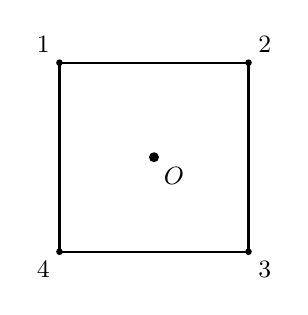
\begin{tikzpicture}[scale=1.2, every node/.style={font=\small}]
    % square centered at origin
    \coordinate (A) at (-1,-1); % 1
    \coordinate (B) at ( 1,-1); % 2
    \coordinate (C) at ( 1, 1); % 3
    \coordinate (D) at (-1, 1); % 4
    \draw[thick] (A) -- (B) -- (C) -- (D) -- cycle;

    % vertex dots + labels
    \fill (A) circle (1pt); \node[below left]  at (A) {4};
    \fill (B) circle (1pt); \node[below right] at (B) {3};
    \fill (C) circle (1pt); \node[above right] at (C) {2};
    \fill (D) circle (1pt); \node[above left]  at (D) {1};

    % origin
    \fill (0,0) circle (1.5pt);
    \node[below right] at (0,0) {$O$};
  \end{tikzpicture}
\end{wrapfigure}

Here is a square centered at the origin. Take a copy of the square, move it around in 3-space, and lay it back down to cover the original square. This is called a rigid motion of the square, or a symmetry of the square. This creates a permutation of the vertices. How many symmetries are possible?

%%%%%%%%%%%%%%%%figures go here %%%%%%%%%%%%%%%%

For the arbitrary symmetry of the square, we have 4 choices where to find 1. Once we know where vertex 1 is (say, vertex i), then vertex 2 can be one of 2 places. This gives $4\times2$ symmetries. Consider the regular $n$-gon centered at the origin. How many symmetries do we have? $2n$.

\begin{fact} [Properties of Permutations] \leavevmode \\
\begin{enumerate}
    \item Functional composition is associative. For mappings $\sigma, \tau, \mu$
    $$\sigma \circ (\tau \circ \mu) = (\sigma \circ \tau) \circ \mu$$
    \item The identity mapping on any set ($I(x) = x$) is a bijection of that set.
    \item If $\sigma$ is a bijection from a set $\Omega$ to $\Omega$, then there is a bijection of $\Omega$ called $\sigma^{-1}$ such that $\sigma \circ \sigma^{-1} = I = \sigma^{-1} \circ \sigma$.
\end{enumerate}
\end{fact}

\begin{definition}[Order] \leavevmode \\
    For $a\in G$, where $G$ is a group, the order of $a$, denoted $|a|$, is the smallest positive integer $k$ such that $a^k = e$ if such a $k$ exists. If no such $k$ exists, then we say $a$ has infinite order and $|a| = \infty$.
\end{definition}

\begin{notation}[Cycle Decomposition] \leavevmode \\
    A permutation $\sigma$ of a set $\Omega$ can be written as a product of disjoint cycles. For example, if $\sigma$ is a permutation of $\{1,2,3,4,5\}$ such that $\sigma(1)=3$, $\sigma(3)=1$, $\sigma(2)=5$, $\sigma(5)=2$, and $\sigma(4)=4$, then we can write $\sigma = (1~3)(2~5)(4)$. The order of a cycle is the number of elements in the cycle. The order of a permutation is the least common multiple of the orders of the disjoint cycles.
\end{notation}

\begin{example} \leavevmode \\
  If $\sigma = (1~2)(3~2),$ then $\sigma(3) = 1$. \\
  If $\mu = (3~2)(1~2),$ then $\mu(3) = 2$. \\
  $S_n$ is not abelian for $n \geq 3$.
\end{example}

\newpage

\section{Orders of Permutations}
$S_X$ refers to the set of all permutations on the set $X$. That is, the elements of $S_X$ are bijections from $X$ to itself. $S_n$ refers to when $X=\set{1,2,\ldots,n}.$

Let $n=5$. How many elements are in $S_5$? $5!=120$. Why? Given a $\sigma \in S_5$, we have $5$ choices for $\sigma(1)$, 4 for $\sigma(2),...$ so there are $5\cdot 4 \cdot 3 \cdot 2 \cdot 1=5! = 120$ choices for $\sigma$. In general, there $n!$ elements in $S_n$.

$S_5:$ how many cycles of length $5$ are in $S_5$?

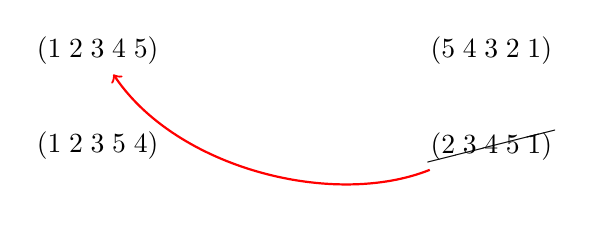
\begin{tikzpicture}[baseline=(current bounding box.center)]
\node (a) at (0,0) {$(1\;2\;3\;4\;5)$};
\node (b) at (5,0) {$(5\;4\;3\;2\;1)$};
\node (c) at (0,-1.2) {$(1\;2\;3\;5\;4)$};
\node (d) at (5,-1.2) {$\cancel{(2\;3\;4\;5\;1)}$};
\draw[->, red, thick] (d) .. controls (3,-2) and (1,-1.5) .. (a);
\end{tikzpicture} 

$\vdots$

There are $5!$ ways of filling in a blank 5-cycle. However, each 5-cycle is represented 5 ways, so we divide by 5. Thus there are $\frac{5!}{5} = 4! = 24$ distinct 5-cycles in $S_5$.How many
\begin{align*}
    \text{4 cycles? } & \frac{5\cdot4\cdot3\cdot2}{4} = 30 \\
    \text{3 cycles? } & \frac{5\cdot4\cdot3}{3} = 20 \\
    \text{2 cycles? } & \frac{5\cdot4}{2} = 10 \\
    \text{1 cycles? } & \frac{5}{1} = 5
\end{align*}

How many distinct $r$-cycles $r \leq n$ are there in $S_n$? $\frac{n!}{r(n-r)!}$
$$\frac{n\cdot(n-1)\cdot(n-2)\cdots(n-r+1)}{r!}$$

How many distinct elements of the form $(\_ \_)(\_ \_ \_)$ disjoint in $S_5$?
$$\frac{5\cdot4}{2} \cdot \frac{3\cdot2\cdot1}{3} = 20$$

How many of the form $(\_ \_)(\_ \_)$?
$$\frac{\frac{5\cdot4}{2} \cdot \frac{3\cdot2}{2}}{2} = \frac{30}{2}=15$$

How many distinct elements of the form $(\_ \_)(\_ \_ \_)$ in $S_n$?
$$\frac{n\cdot(n-1)}{2} \cdot \frac{(n-2)(n-3)(n-4)}{3}$$

How many distinct elements of the form $(\_ \_)(\_ \_)$ in $S_n$?
$$\frac{\frac{n\cdot(n-1)}{2} \cdot \frac{(n-2)(n-3)}{2}}{2}$$

\begin{definition}[Field] \leavevmode \\
    $(F, +, \cdot)$ is a field if
    \begin{enumerate}
        \item $(F, +)$ is an abelian group with identity $0$
        \item $(F\setminus\set{0}, \cdot)$ is an abelian group with identity $1$
        \item Left and right distributive laws hold
    \end{enumerate}
\end{definition}

The following are groups:
\begin{align*}
    GL_n(F) &= \set{\text{all $n\times n$ matrices with entries in $F$ and with non-zero determinants}} \\
    SL_n(F) &= \set{\text{all $n\times n$ matrices with entries in $F$ and with determinant $1$}}
\end{align*}
\newpage

\section{Homomorphism and Isomorphism}
In general, we can tell how similar groups are by the mappings we make between them where the mappings preserve the group structure of the domain.

\begin{definition}[Homomorphism] \leavevmode \\
    Let $(G, \star)$ and $(H, \diamond)$ be groups. A map $\Phi: G \to H$ is a homomorphism if for all $g_1, g_2 \in G$,
    $$\Phi(g_1 \star g_2) = \Phi(g_1) \diamond \Phi(g_2)$$
    We usually write
    $$\Phi(xy) = \Phi(x) \Phi(y)$$
    and we know that $xy$ happens in $G$ and $\Phi(x)\Phi(y)$ happens in $H$.
\end{definition}

\begin{example}
    $\pi: \R^2 \to \R$ by $\pi(x,y) = x$ $\forall (x,y) \in \R^2$ is a homomorphism. Letting $(x_1, y_1), (x_2, y_2) \in \R^2$, we have
    \begin{align*}
        \pi((x_1, y_1) + (x_2, y_2)) &= \pi(x_1 + x_2, y_1 + y_2) \\
        &= x_1 + x_2 \\
        &= \pi(x_1, y_1) + \pi(x_2, y_2)
    \end{align*}
    Showing that $\pi$ is indeed a homomorphism.

    What elements are in the set $\set{p \in \R^2 : \pi(p) = 0} = K$?
    $$K = \set{(x,y) : x=0}$$
    This is the kernel of $\pi$.
\end{example}

\begin{definition}[Kernel] \leavevmode \\
    Let $G$ and $H$ be groups and let $\Phi: G \to H$ be a group homomorphism. The kernel of $\Phi$ is
    $$\ker(\Phi) = \set{g \in G : \Phi(g) = e_H} = \Phi^{-1}(e_H)$$
    where $e_H$ is the identity element in $H$.
\end{definition}

\begin{definition}[Isomorphism] \leavevmode \\
    Let $G$ and $H$ be groups. A map $\Psi: G \to H$ is an isomorphism if
    \begin{enumerate}
        \item $\Psi$ is a homomorphism
        \item $\Psi$ is bijective
    \end{enumerate}
    If there exists an isomorphism $\Psi: G \to H$, we say that $G$ and $H$ are isomorphic, denoted $G \cong H$.
    
    $\cong$ is an equivalence relation on any collection of groups.
\end{definition}

\begin{example}
    Let $k \in \Q^\ast = \Q \setminus \set{0}$. Define $\phi_k: \Q^\ast \to \Q^\ast$ by $\phi_k(q) = kq$. We claim that $\phi$ is an isomorphism.
    Show that $\Phi_k$ is a homomorphism and a bijection:
    \begin{enumerate}
        \item Homomorphism:
        \begin{align*}
            \phi_k(q_1 + q_2) &= k(q_1 +q_2) \\
            &= k (q_1+ q_2) \\
            &= kq_1 + kq_2 \\
            &= \phi_k(q_1) + \phi_k(q_2)
        \end{align*}
        \item Bijections:
        \begin{itemize}
            \item Injective: Suppose $\phi_k(q_1) = \phi_k(q_2)$. Then \begin{align*}
                \phi_k(q_1) &= \phi_k(q_2) \\ \iff
                kq_1 &= kq_2 \\ \iff
                q_1 &= q_2 &&(k \neq 0)
            \end{align*}
            \item Surjective: We want to show $\phi_k(\Q) = \Q$. Let $q \in \Q.$ Since $k \neq 0$, $\frac{q}{k} \in \Q$. Then
            $$\phi_k\left(\frac{q}{k}\right) = k \cdot \frac{q}{k} = q$$
            Thus $\phi_k$ is surjective.
        \end{itemize}
    \end{enumerate}
    ker$\phi_k=\set{0}$ since $\phi_k(q) = 0 \iff kq = 0 \iff q=0$.
\end{example}

\begin{fact}
    Suppose $G \cong H,$ that is there exists $\phi: G \to H$ which is a homomorphic bijection. Then
    \begin{enumerate}
        \item $|G|=|H|$
        \item $G$ is abelian if and only if $|H|$ is abelian
        \item $\forall x \in G ~~|x| = |\phi(x)|$ (Corresponding elements have the same order)
    \end{enumerate}
\end{fact}
\newpage

\section{Group Actions}
There are many examples of groups acting on sets. For instance, consider an element in $S_5$, call it $\sigma.$ $\sigma$ is a permutation of $\set{1,2,3,4,5}$ and it is also an element of a group
\begin{align*}
    \sigma &= (1~2~3~4~5) \\
    &\sigma(5) = 4
\end{align*}
We say that $\sigma$ is acting on the set $\set{1,2,3,4,5}$.

Consider the set of all $2\times 2$ matrices with elements in $\R$. Let $A = \begin{bmatrix}
1 & 2 \\
3 & 4
\end{bmatrix}$ and let $k \in \R.$ Then $kA = \begin{bmatrix}
k & 2k \\
3k & 4k
\end{bmatrix}.$ We say that $\R$ is acting on the set of all $2\times 2$ matrices with elements in $\R$.

\begin{definition}[Group Action] \leavevmode \\
    Let $G$ be a group and $A$ be a set. A group action of $G$ on $A$ is a map from $G\times A$ to $A$ (written $g.a ~~\forall g \in G, a \in A$) such that
    \begin{enumerate}
        \item $g_1.(g_2.a) = (g_1g_2).a ~~\forall g_1, g_2 \in G$ (Compatability)
        \item $1.a = a$ (or $e.a = a$) $ ~~\forall a \in A$ (Identity)
    \end{enumerate}
\end{definition}

\begin{example}
    Let $G = S_n$. Let's verify that $S_n$ acts on the set $\set{1,2,...,n}.$ Define the group action
    \begin{align*} \tag{$*$}
        \sigma.a = \sigma(a) ~~\forall \sigma \in S_n, a \in \set{1,2,...,n}
    \end{align*}
    Then let $\sigma_1, \sigma_2 \in S_n$ and $a \in \set{1,2,...,n}.$ We have
    \begin{align*}
        \sigma_1.(\sigma_2.a) &= \sigma_1.(\sigma_2(a)) \\
        &= \sigma_1(\sigma_2(a)) \\
        &= (\sigma_1\circ\sigma_2)(a) \\
        &= (\sigma_1\circ\sigma_2).a \tag{I}
    \end{align*}
    To verify the identity property, recall that the identity map, denoted $I$, is the identity of $S_n$ and $$I(a) = a ~~\forall a \in \set{1,2,...,n}$$
    That is,
    \begin{align*}
        I.a = I(a) = a ~~\forall a \in \set{1,2,...,n} \tag{II}
    \end{align*}
    By $(I)$ and $(II)$, $S_n$ acts on the set $\set{1,2,...,n}$ by the group action defined in $(*)$.
\end{example}

\begin{example}
    A vector space over a field $F$ is a set $V$ with two binary operations vector addition and scalar multiplication, and other poperties including 
    \begin{itemize}
        \item $a(bv) = (ab)v ~~\forall a, b \in F, v \in V$ (Compatability)
        \item $1v = v ~~\forall v \in V$ where $1$ is the multiplicative identity in $F$ (Identity)
    \end{itemize}
    Since $F$ is not a group with respect to multiplication, we must say that $F^\ast = F \setminus \set{0}$ acts on $V$.
\end{example}
\newpage

\section{Permutations and Group Actions}
Let $G$ be a group acting on a set $S$. That is, define a mapping $G \times S \to S$ denoted by $g.a ~~\forall g \in G$ and $a \in S$. Fix $g \in G.$ Then this defines a map $\sigma_g \st \sigma_g : S \to S$ by $\sigma_g (a) = g.a$

\begin{example}
    Take $G = \R \setminus \set{0}$ with respect to multiplication. Let $S = M_2(\R)$.
    \begin{align*}
        \sigma_{\sqrt{2}}(A) &= \sqrt{2}.A \\
        &= \sqrt{2} \begin{bmatrix}
            a & b \\
            c & d
        \end{bmatrix} \\
        &= \begin{bmatrix}
            \sqrt{2}a & \sqrt{2}b \\
            \sqrt{2}c & \sqrt{2}d
        \end{bmatrix}
    \end{align*}
    For $\begin{bmatrix}
        1 & \pi \\
        e & \ln(2)
    \end{bmatrix}$, we have
    \begin{align*}
        \sigma_{\sqrt{2}} \begin{bmatrix}
            1 & \pi \\
            e & \ln(2)
        \end{bmatrix} &= \begin{bmatrix}
            \sqrt{2} & \sqrt{2}\pi \\
            \sqrt{2}e & \sqrt{2}\ln(2)
        \end{bmatrix}
    \end{align*}
    What is the range of $\sigma_{\sqrt{2}}$? $M_2(\R)$.
\end{example}

\begin{assertion}
    \begin{enumerate}
        \item $\sigma_g$ as defined is a permutation of the set $S$.
        \item For the sake of notation, we change the name of our set to $A$. The map from $G$ to $S_A$ defined by $g \mapsto \sigma_g$ is a homomorphism.
    \end{enumerate}
\end{assertion}

\begin{proof}
    \begin{enumerate}
        \item Let $g\in G$ be given and $\sigma_g$ be defined as above. Clearly, $\sigma_g$ is a mapping from $S \to S$. We will show that $\sigma_g$ is a bijection by showing it has a two-sided inverse. Let $a \in S$ and note $g^{-1}\in G$ since $G$ is a group. Then
        \begin{align*}
            \left(\sigma_{g^{-1}} \circ \sigma_g \right)(a) &= \sigma_{g^{-1}}(\sigma_g(a)) \\
            &= \sigma_{g^{-1}}(g.a) \\
            &= g^{-1}.(g.a) \\
            &= (g^{-1}g).a \\
            &= e.a \\
            &= a.
        \end{align*}
        We see that $\sigma_{g^{-1}} \circ \sigma_g$ is the identity mapping from $S \to S$. To show that $\sigma_g \circ \sigma_{g^{-1}}$ is also the identity map from $S \to S$ is analogous. Thus we have a two-sided inverse as desired. Hence, $\sigma_g$ is a permutation of $S$ as desired. That is, $\sigma_g$ is an element of the symmetric group of $S$.

        \item Let $\Psi: G \to S_A$ be defined by $\Psi(g) = \sigma_g ~~\forall g \in G$. Let $a \in A$ and $g_1, g_2 \in G$. We want to show that $\Psi(g_1g_2) = \Psi(g_1) \circ \Psi(g_2)$. Since these are mappings in $S_A$, we will show that their values agree $\forall a \in A$. We have
        \begin{align*}
            \left(\Psi(g_1) \circ \Psi(g_2)\right)(a) &= \sigma_{g_1g_2}(a) \\
            &= (g_1g_2).a \\
            &= g_1.(g_2.a) \\
            &= g_1.(\sigma_{g_2}(a)) \\
            &= \sigma_{g_1}(\sigma_{g_2}(a)) \\
            &= \sigma_{g_1} \circ \sigma_{g_2}(a) \\
            &= \left(\Psi(g_1) \circ \Psi(g_2)\right)(a).
        \end{align*}
        Hence, $\Psi$ is a homomorphism as desired.
    \end{enumerate}
    \qed
\end{proof}

If we have a homomorphism, then we have a kernel.

\begin{definition}[Kernel of a Group Action] \leavevmode \\
    For a group $G$ acting on a set $A$, the kernel of the group action is
    $$\set{g \in G : g.a = a ~~\forall a \in A}$$
\end{definition}
\newpage

\chapter{Subgroups}
\section{Subgroups}
\begin{definition} [Subgroup] \leavevmode \\    
    Let $G$ be a group. The subset $H$ of $G$ is called a subgroup of $G$ if 
    \begin{enumerate}
        \item $H$ is nonempty.
        \item $\forall x,y \in H$, $x^{-1} \in H$ and $xy \in H$.
    \end{enumerate}
\end{definition}

\begin{notation}
    IF $H$ is a subgroup of $G$, we write $H \leq G$.
\end{notation}

\begin{example} \leavevmode \\
    \begin{enumerate}
        \item $\Z \leq \Q$ with respect to $(+)$.
        \item All groups have two subgroups: $H=G$ and $H=\set{1}$.
        \item $2\Z \leq \Z$ with respect to $(+)$.
        \item Let $G=D_{2n}$ and let $r$ be a $360^{\circ}/n$ clockwise rotation of the n-gon about the origin. Then $\set{1, r, r^2, r^3,...,r^{n-1}}$ forms a subgroup of $D_{2n}$.
        \item Nonexample: $H=\set{1, -1} \subseteq \Z$ forms a group with respect to multiplicaiton, but $H$ is not a subgroup of $\Z$ since $\Z$ is a group with respect to addition, NOT multiplicaiton.
        \item $\Z/5\Z$ is not a subgroup of $\Z/6\Z$ since $\Z/5\Z \not \subseteq \Z/6\Z$.
        \begin{align*}
            \Z/6\Z &= \set{\bar{0}, \bar{1}, \bar{2}, \bar{3}, \bar{4}, \bar{5}} \text{ is an additive group} \\
            \left(\Z/6\Z\right)^* &= \set{\bar{1}, \bar{5}} \text{ is a multiplicative group with all elements coprime to 6} \\
            \left(\Z/9\Z\right)^{**} &= \set{\bar{1}, \bar{2}, \bar{4}, \bar{5}, \bar{7}, \bar{8}} \text{ is a multiplicative group with all elements coprime to 9}
        \end{align*}
    \end{enumerate}
\end{example}

\begin{proposition}[Subgroup Criterion] \leavevmode \\
    A subset $H$ of a group $G$ is a subgroup of $G$ if and only if
    \begin{enumerate}
        \item $H\not = \emptyset$.
        \item $\forall x,y \in H$, $xy^{-1} \in H$ (in additive notation: $\forall x,y \in H$, $x-y \in H$).
    \end{enumerate}
\end{proposition}
\newpage

\section{Centralizers and Normalizers, Stabilizers and Kernels}
\begin{definition} [Centralizers] \leavevmode \\
    Let $A$ be a nonempty subset of a group $G$. Define the centralizer of $A$ in $G$ to be the set
    \begin{align*}
        C_G(A) &= \{ g \in G : gag^{-1} = g ~~\forall a \in A \} \\
        &= \set{g \in G : ga = ag ~~\forall a \in A}
    \end{align*}
\end{definition}

The centralizer of $A$ in $G$ is the set of all elements in $G$ which commute with every element in $A$.

\begin{theorem}
    $C_G(A) \leq G$.
\end{theorem}

\begin{proof}
    Let $a \in A.$ Then 
    \begin{align*}
        1a1^{-1} &= (1a)1^{-1} \\
        &= a1^{-1} \\
        &= a1 \\
        &= a
    \end{align*}
    Thus, $1 \in C_G(A)$.

    Let $x,y \in C_G(A)$. Then $xax^{-1} = a$ and $yay^{-1}=a.$ Note that
    \begin{equation*}
        yay^{-1} = a \iff a = y^{-1}
        \tag{$*$}
    \end{equation*}
    Now
    \begin{align*}
        (xy^{-1})a(xy^{-1})^{-1} &= xy^{-1}a(y^{-1})^{-1}x^{-1} \\
        &= x(y^{-1}ay)x^{-1} \\
        &\overset{(*)}{=} xax^{-1} \\
        &= a
    \end{align*}
    Hence, $xy^{-1} \in C_G(A)$. Furthermore, $C_G(A) \leq G.$
    \qed
\end{proof}

\begin{notation}
    If $A = \set{a}$, we write $C_G(a)$ instead of $C_G(\set{a})$.
\end{notation}

Why was this unnecessary? From the homework, we know that $G$ acts on the subset $A$ by conjugation. That is, we have a mapping $(.): G\times A \to A$ defined by $g.a = gag^{-1} ~~\forall g \in G, a \in A$ which satisfies both axioms of a group action.

Recall that the kernel of a group action is the kernel of the permutation representation of the group action (PRGA). The PRGA is the Homomorphism induced by the group action
\begin{align*}
    \Psi : G \to S_A \\
    g \mapsto \sigma_g
\end{align*}

\begin{example}
    Find the kernel of $G$ acting on $A \subset G$ by conjugation.
    \begin{align*}
        \set{g \in G : g.a = a ~~ \forall a \in A} &= \set{g \in G : gag^{-1} = a ~~\forall a \in A} \\
        &= C_G(A)
    \end{align*}
\end{example}

Suppose that $A = G$. What is $C_G(G)$?
$$\set{g \in G : gag^{-1}=a ~~\forall a \in G}$$
This set is called the center of $G$ denoted $Z(G)$. Since $Z(G)$ is a special case of $C_G(A)$, we know $Z(G) \leq G$.

\begin{definition}[Normalizer] \leavevmode \\
    Define $gAg^{-1} = \set{gag^{-1} : a \in A}$. We will define the normalizer of $A$ in $G$ to be the set 
    $$N_G(A) = \set{g \in G : gAg^{-1} = A}$$
\end{definition}

We will prove $N_G(A) \leq G$, but not yet.
Notice if $gag^{-1} = a ~~ \forall a \in A$ then $gAg^{-1} = \set{gag^{-1} : a \in A} = \set{a : a \in A} = A$. Hence
$$C_G(A) \subseteq N_G(A)$$

\begin{fact} \leavevmode \\
    \begin{enumerate}
        \item If $G$ is abelian, then $Z(G) = G$ since every element commutes with every other element. That is,
        \begin{align*}
        \forall a,b \in G ~~ab = ba &\iff a = bab^{-1} ~~ \forall a,b \in G \\ &\implies b \in Z(G) ~~\forall b \in G
        \end{align*}
        Similarly, $C_G(A) = N_G(A) = G.$
        \item Consider $A=\set{1, (1 ~2)} \subseteq S_3$. Find $C_{S_3}(A)$. Notice that $1$ commutes with everything in $S_3$, specifically $1$ and $(1~2)$. Also,
        $$(1~2)(1~2)(1~2)^{-1} = (1~2)$$
        so $(1~2)\in C_{S_3}(A)$. Hence, $A \leq C_{S_3}(A)$.
        \begin{theorem}[Lagrange's Theorem] \leavevmode \\
            Let $G$ be a finite group $\left(|G| \in \N\right)$ and let $H \leq G$. Then
            $$|H| \text{ divides } |G|$$
        \end{theorem}
        Since $|A| = 2$ and $A \leq C_{S_3}(A)$, we know $2 \big| |C_{S_3}(A)|$ since $C_{S_3}(A) \leq S_3$.
        $$
        \begin{rcases*}
            |C_{S_3}(A)| \big| |S_3| = 3! = 6 \\
            |A| \big| |C_{S_3}(A)|
        \end{rcases*} \implies |C_{S_3}(A)| \in \set{2, 6}$$.
        Thus, $C_{S_3}= A$ or $C_{S_3}(A) = S_3$. Well,
        \begin{align*}
            (1~2)(1~2~3) = (2~3) \\
            (1~2~3)(1~2) = (1~3)
        \end{align*}
        so $(1~2~3) \not \in C_{S_3}(A)$. It follows that $|C_{S_3}(A)| = 2 \implies C_{S_3}(A) = A.$
    \end{enumerate}
\end{fact}
\newpage

\section{Cyclic Groups}
\begin{definition}[Cyclic Group] \leavevmode\\
    A group $H$ is cyclic if $H$ is generated by a single element. That is,
    $$\exists x \in H \st H = \set{x^n : n \in \Z}$$
    $$\left(\exists x \in H \st H = \set{nx : n \in \Z} \text{ using additive notation}\right)$$
    We write $<x> = H$ ($x$ generates $H$).
\end{definition}

\begin{example}
    \begin{enumerate}
        \item $\Z=<1>=<-1>$
        \item The rotations in $D_{2n}$ are generated by $r$ ($360/n$ clockwise rotation)
        \item $U_4 = {1, -1, i, -i} = <i>$
    \end{enumerate}
\end{example}

\begin{note}
    If $H=<x> = \set{x^n : n \in \Z}$, we define 
    \begin{align*}
        x^0 &= 1 \\
        x^{-n} &= (x^n)^{-1} = (x^{-1})^n \text{ for } n > 0
    \end{align*}
\end{note}

\begin{proposition}
    If $H=<x>$, then $|H| = |x|$. If one side of this equality is infinity, then so is the other. More specifically,
    \begin{enumerate}
        \item If $|x| = n < \infty$, then $x^n = 1$ and $1, x, x^2, ..., x^{n-1}$ are all the distinct elements of $H$.
        \item If $|x| = \infty$, then $x^n \not = 1$ when $n \not = 0$ and $x^a \not = x^b$ for all $a \not = b \in \N$.
    \end{enumerate}
\end{proposition}

\begin{proof}
    Let $|x| = n$.
    \begin{enumerate}
        \item Consider the case where $n < \infty$. Consider the elements $1, x, x^2, ..., x^{n-1}$ and suppose $x^a = x^b$ where $0 \leq a < b < n$. Then 
        \begin{align*}
            x^a = x^b &\implies 1 = x^bx^{-a} \\
            &\implies 1 = x^{b-a}
        \end{align*}
        Since $b-a > 0$, this contradicts $n$ being the order of $x$. Thus, all the $1, x, x^2, ..., x^{n-1}$ are distinct. Also, $x^n = 1$ as $n = |x|$. Thus $H$ contains at least $n$ elements. It remains to show we have all of them. \\
        Let $t \in Z \st x^t \in H$. By the division algorithm, there exitst $q, r \in \Z$ such that 
        $$t = qn + r \text{ where } 0 \leq r < n$$
        Then
        \begin{align*}
            x^t = x^{qn+r} &= x^{qn}x^r \\
            &= (x^n)^qx^r \\
            &= 1^q x^r \\
            &=x^r \in \set{1, x, x^2, ..., x^{n-1}} \text{ since } 0 \leq r < n
        \end{align*}
        Hence, $H = \set{1, x, x^2, ..., x^{n-1}}$.

        \item Next, suppose $|x| =\infty$ (no positive powers of $x$ is the identity). For the sake of contradiction, if $x^a=x^b$ with $a < b$ then $x^{a-b}=1$, a contradiction. So distinct powers of $x$ give distinct elements of $H$. It follows that $|H| =\infty$.
    \end{enumerate}
    \qed
\end{proof}

\begin{proposition}
    Let $G$ be a group and let $x \in G$. Let $m,n \in \Z.$ If $x^n = 1$ and $x^m = 1,$ then $x^d = 1$ where $d = \gcd (m,n).$ In particular, if $x^m = 1$ for some $m \in \Z$ then $|x| | m$.
\end{proposition}

\begin{proof}
    Let $m, n, d$ be defined as above. Then by the Euclidean algorithm
    $$\exists x_0, y_0 \in \Z \st d = mx_0 +ny_0$$
    Then 
    \begin{align*}
        x^d &= x^{mx_0 + ny_0} \\
        &= (x^m)^{x_0}(x^n)^{y_0} \\
        &=1^{x_0}1^{y_0} \\
        &=1
    \end{align*}
    To prove the second assertion, let $x^m = 1$ and $n = |x|$. Then $x^n = 1$ by definition of order.
    \begin{description}
        \item[Case 1: ] If $m = 0$ then certainly $n | m$.
        \item[Case 2: ] Let $m \not = 0$. We know $n < \infty$ since $x^m = 1$. Let $d = \gcd(m,n)$ and hence by the first assertion $x^d = 1$. Since $0 < d \leq n$ and $n$ is the smallest positive integer such that $x^n = 1$, we have that $n = d.$ By definition,
        $$d | m \implies n | m \text{ as desired.}$$
    \end{description}
    \qed
\end{proof}

\begin{theorem}[Cyclic Groups Isomorphisms] \leavevmode\\
    \begin{enumerate}
        \item Any infinite cyclic group $<x>$ is isomorphic to $\Z$ (with the mapping $\phi : \Z \to <x>$, $k \mapsto x^k$).
        \item If $<x>$ and $<y>$ are cyclic groups both with order $n < \infty$, then
        \begin{align*}
            \phi: <x> &\to <y> \\
            x^k &\mapsto y^k
        \end{align*}
        is a well-defined isomorphism.
    \end{enumerate}
\end{theorem}

We will use multiplicative notation when describing an arbitrary cyclic group of order $n \in \N$, and denote this group $\Z_n.$ NOT to be confused with the additive group $\Z/n\Z$, which is cyclic of order $n$. Most times we will refer to an infinite cyclic group as $\Z$.

\begin{proposition}[The Order of $x^a$ in a Cyclic Group] \leavevmode\\
    \label{prop5}
    Let $G$ be a group and let $x \i9n G$. Let $a \in \Z-\{0\}.$
    \begin{enumerate}
        \item If $|x| = \infty,$ then $|x^a| = \infty$.
        \item If $|x| = n < \infty,$ then $|x^a| = \frac{n}{\gcd(n,a)}$.
    \end{enumerate}
    In particular, $|x^a| = \frac{n}{a}$ when $a|n$ ($a \in \N$).
\end{proposition}

\begin{proof}
    We start with the following claim: Let $a,n, \in \Z$ not both zero.
    $$\text{If $\gcd(a,n) = d$ then $\gcd(\frac{a}{d}, \frac{n}{d})=1$}$$

    \begin{proof}
        Let $a,n$ and $d$ be as defined. Then there exists $x_0, y_0 \in Z$ such that 
        $$d = ax_0 + ny_0$$
        It follows that
        $$1 = \frac{a}{d}x_0 + \frac{n}{d}y_0$$
        Since $\gcd(\frac{a}{d}, \frac{n}{d})$ divides $\frac{a}{d}$ and $\frac{n}{d}$, $\gcd(\frac{a}{d}, \frac{n}{d})$ divides the right-hand side, so $\gcd(\frac{a}{d}, \frac{n}{d}) | 1$. Thus, $\gcd(\frac{a}{d}, \frac{n}{d}) = 1$.
        \qed
    \end{proof}
    \begin{enumerate}
        \item Suppose by way of contradiction that 
        $$|x| = \infty \text{ and } |x^a| = m < \infty$$
        By definition of order
        $$(x^a)^m = 1 \iff x^{am} = 1$$
        It follows that
        $$(x^{am})^{-1} = 1^{-1} \iff x^{-am} = 1$$
        Since $a \not = 0$ by assumption and $m \not = 0$ by definition of order, then $am \not = 0$ and one of $-am$ or $am$ is positive, so some positive power of $x$ is the identity, contradicting $|x| = \infty.$ So, $|x^a| = \infty$.

        \item Let $|x| = n < \infty$ and let $y = x^a$, $\gcd(a,n) = d$. We also write $n = db$ and $a = dc$ for some integers $c, b$ (not thate $ b > 0$). From our claim,
        $$\gcd(c,b) = \gcd(\frac{a}{d}, \frac{n}{d}) = 1$$
        We want to show that $|y| = b$. To this end, cotice that
        \begin{align*}
            y^b = (x^a)^b &= x^{ab} \\
            &= x^{(dc)b} \\ 
            &= x^{(dc)(\frac{n}{d})} \\
            &= (x^n)^c \\ 
            &= 1^c \\
            &= 1
        \end{align*}
        Thus, $|y|$ divides $b$. Let $k = |y|$. Then 
        $$y^k = 1 = x^{ak}$$
        Hence, $|x| \mid ak$. That is, 
        \begin{align*}
            n \mid ak &\iff db \mid dck \\
            &\iff b \mid ck \\
            &\iff \frac{n}{d} \mid \frac{a}{d}k
        \end{align*}
        Since $\frac{n}{d}$ and $\frac{a}{d}$ are relatively prime, this gives $\frac{n}{d} \mid k$, that is $b \mid k$. Since $b \mid k$ and $k \mid b$, $k = b$ as both $k,b \in \N$.
        \qed
    \end{enumerate}
\end{proof}

\begin{proposition}
    Let $H = <x>$.
    \begin{enumerate}
        \item Assume $|x| = \infty.$ then $H = <x^a>$ if and only if $a = \pm 1$.
        \item Assume $|x| = n \infty$. Then $H = <x^a>$ if and only if $\gcd(a,n) = 1$. In particular, the number of generators of $H$ is $\phi(n)$, where $\phi$ is Euler's Phi funciton.
    \end{enumerate}
\end{proposition}

\begin{proof}
    2. If $|x| = n < \infty$, we know that $|x^a| = |<x^a>|.$ This subgroup equals all of $H \iff |x^a| = n \iff \frac{n}{\gcd(a,n)}=n \iff \gcd(a,n) = 1.$ Since $\phi(n)$ is the number of $a \in \set{1, 2, 3,..., n}$, which are relatively prime to $n$, $\phi(n)$ gives the number of generators of $H$.
    \qed
\end{proof}

What are the generators of $<x> = \Z_{10}$? $\phi(1) = \phi(2)\phi(5) = 4$
$$x^1, x^3, x^7, x^9$$
What are the generators of $\Z/15\Z = <\overline{1}> = \set{k\dot 1 : k \in \Z}$?
$$\overline{1}, \overline{2}, \overline{4}, \overline{7}, \overline{8},\overline{11},\overline{13},\overline{14}$$

\begin{theorem}[Subgroups of Cyclic Groups] \leavevmode\\
    Let $H=<x>$ be a cyclic group.
    \begin{enumerate}
        \item Every subgroup of $H$ is cyclic. More precisely, if $K \leq H$ then either
        $$K = \set{1} \text{ or } K = <x^d>$$
        where $d$ is the smallest positive integer such that $x^d \in K$.
        \item If $|H| = \infty$, then for any distinct nonnegative integers $a$ and $b$
        $$<x^a> \not = <x^b>$$
        and $\forall m \in \Z$
        $$<x^m> = <x^{|m|}>$$
        where $|m|$ denotes the absolute value of $m$. So, the nontrivial subgroups of $H$ correspond bijectively with the integers $1, 2, 3, ...$
        \item If $|H| = n < \infty$, then for every $a \in \N$ which divides $n$, there is a unique subgroup $H$ with order $a$. This subgroup is the cyclic group $<x^d>$ where $d = \frac{n}{a}$. Furthermore, for every $m \in \Z$, $<x^m> = <X^{\gcd(n,m)}>$ so the subgroups of $H$ correspond bijectively with the positive divisors of $n$.
    \end{enumerate}
\end{theorem}

\begin{proof}
    \begin{enumerate}
        \item Let $K \leq H$. If $K = \set{1}$, then we are done. Suppose $K \not = \set{1}$. Thus, there exists some $a \not = 0 \st x^a \in K$. Since $K$ is a group, $(x^a)^{-1} \in K.$ That is, $x^{-a} \in K$, and since either $a$ or $-a$ must be positive the set of all positive powers of $x \st x$ to that positive power is an element of $K$ is nonempty. That is,
        $$P = \set{n \in \N : x^n \in K} \not = \emptyset$$
        Thus, by the well-ordering principle, the set $P$ contains a minimal element, call it $d$. By definition, $x^d \in K.$ and since $K$ is a group $<x^d> \leq K.$ Let $k \in K.$ Then, $k = x^b$ for some $b \in \Z.$ By the division algorithm, we have integers $q,r$, such that
        $$b = qd +r \text{ where }0 \leq r < d$$
        Hence,
        \begin{align*}
            &x^b = x^{qd+r} \\
            \implies &x^b = (x^{qd})x^r = (x^d)^qx^r \\
            \implies (x^d)^{-q}&x^b = x^r
        \end{align*}
        Since $x^d, x^b \in K$ and $K$ is a group,
        $$(x^d)^{-q} \in K \text{ and } (x^d)^{-q}x^b \in K$$
        so $x^r \in K$. However, since $d$ is the minimal positive power of $x$ such that $x^d \in K$, $r$ must not be a positive power. Therefore, $r = 0$ and it follows that
        $$k = x^b = (x^d)^q \in <x^d>$$
        Therefore, $K \leq <x^d>.$ This gives $<x^d> = K$.

        \item Suppose $|H| = n < \infty$ and $a \mid n$ where $a \in \Z$. Let $d = \frac{n}{a}$. Hence
        $$|<x^d>| = \frac{n}{n/a} = a$$

        \begin{description}
            \item[Uniqueness: ] To show uniqueness, suppose $K$ is any subgroup of $H$ of order $a$. Then by part 1, $K = <x^b>$ where $b$ is the smallest positive integer such that $x^b \in K$. We know
            $$\frac{n}{d} = a = |K| = |x^b| = \frac{d}{\gcd(n,b)}$$
            It follows that 
            $$d = \gcd(n,b)$$
            Hence, $d \mid b$ by definition and $x^b \in <x^d>$. It follows that 
            $$K = <x^b> \leq <x^d>$$
            and so $K = <x^d>$ as they have the same order. The final assertion follows from the fact that 
            $$<x^m> \leq <x^{\gcd(m,n)}>$$
            and \ref{prop5} (2) says
            $$\left|<x^m>\right| = \frac{n}{\gcd(n,m)}$$
            and
            $$\left|x^{\gcd(m,n)}\right|=\frac{n}{\gcd(n, \gcd(m,n))}$$
            and we know $\gcd(n, \gcd(m,n)) = \gcd(n,m)$. Since $\gcd(,m,n) \mid n$ this shows that every subgroup of $H$ arises from a divisor of $n$.
            \qed
        \end{description}
    \end{enumerate}
\end{proof}
\newpage

\section{Subgroups Generated by Subsets of a Group}
We have already examined the case of generating a subgroup with one element ($<x>)$. What does it mean to generate a subgroup or a group with more than one element?

\begin{example}
    $D_{2n} = $ symmetries of a regular n-gon centered around the origin. Let $r$ be a $360/n$ clockwise rotation of the n-gon about the origin. Let $S$ be a reflection of the n-gon about the line from vertex $1$ to the origin.

    \includegraphics[width= 100pt, center]{/Users/josiahvillarante/GradSchool/Grad-School-Notes/Math210A/CH2/images/Symmetry over vertex 1.png}

    Notice: $1, r, r^2, r^3$ are all distinct. Now consider $s, sr, sr^2, sr^3$ (we read these right-to-left). $sr^3$ is the $270^\circ$ rotation clockwise, then the reflection about the line where vertex $1$ was to the origin.

    \includegraphics[width= 100pt, center]{/Users/josiahvillarante/GradSchool/Grad-School-Notes/Math210A/CH2/images/sr^3.png}

    Is $s \in \set{1, r, r^2, r^3}?$ No, $s$ fixes vertex $1$ and the only element that fixes vertex $1$ is the identity. But $s \not = 1$, so $s$ is not a rotation. From here, we can deduce that
    $$sr^j \not r^i$$
    for any $0 \leq j \leq 3$ or $0 \leq i \leq 3$ (if it were true that $sr^j = r^i$ for some $i$ and $j$, then $s = r^{i-j}$). Hence $D_{2\dot 4} = \set{1, r, r^2, r^3, s, sr, sr^2, sr^3} = <r, s>/$
\end{example}

In $D_{2n}, n \geq 3,$ we want to show that 
$$D_{2n} = \set{e, r, r^2, r^3, ..., r^{n-1}, s, sr, sr^2, ..., sr^{n-1}}$$
where $s$ is a reflection over the line passing through vertex $1$ and the origin.

\includegraphics[width= 100pt, center]{/Users/josiahvillarante/GradSchool/Grad-School-Notes/Math210A/CH2/images/n-gon reflection.png}

\begin{enumerate}
    \item Why are all $e, r, r^2, ..., r^{n-1}$ distinct? 
    \begin{align*}
        r^i(1) &= i + 1 \text{ for $0\leq i \leq n -1$ } \\
        r^i(1) &= r^j(1) \\
        \implies i + 1 &= j + 1 \\
        \implies i &= j
    \end{align*}
    so the $r^i$'s are distinct.

    \item $s \not = r^i$ for any $i \in \set{0, ..., n-1}$. $s(1) = 1$ if $r^i(1) = 1,$ we know from part 1 that $i = 0$. That is, $r^i = e$. But $s(2) = n \not = 2 = e(2) \implies s \not = e, s \not = r^i ~\forall 0 \leq i \leq n$

    \item Let's show that $r^i \not = sr^j$ for any $i, j \in \set{0, ..., n-1} = A$.
    Suppose there exists $i,j\in A \st r^i = sr^j$. We define $r^{-1}$ as a counter-clockwise rotation; $r^-1 = r^{n-1}$. This gives 
    \begin{align*}
        r^i &= sr^j \\
        \implies r^{i-j} &= s \\
        \implies r^{i + n-j} &= s
    \end{align*}
    where we adjust $(i + n-j) \mod n$ as needed. This contradicts $s \not \in \set{e, r, r^2, ..., r^{n-1}}$. Hence $r^i \not = sr^j$ for any $i, j \in A$.

    \item Show that $sr^i \not = sr^j$ for any $i \not = j$ in $A$.
    For the sake of contradiction, suppose there exists $i, j \in A \st sr^i = sr^j.$ Then 
    \begin{align*}
        s^2r^i &= s^2r^j \\
        \implies er^i &= er^j \\
        \implies r^i &= r^j
    \end{align*}
    This contradicts $i \not = j$.
    \begin{align*}
        &D_{2n} = \set{e, r, r^2, ..., r^{n-1}, s, sr, sr^2, ..., sr^{n-1}} \\ 
        &sr \not = rs \\
        (s\circ r)(1)=s(r(1)) &&(r \circ s)(1)=r(s(1)) \\
        = s(2)  &&= r(1)  \\
        = n  &&= 2
    \end{align*}
    But $sr = r^{-1}s$. If $sr(1) = r^{-1}s(1)$ and $sr(2) = r^{-1}s(2),$ then $sr = r^{-1}s.$ It can be shown inductively that $sr^i = r^{-i}s ~\forall i \in \Z.$
\end{enumerate}

Let $ x\in G$ and $H \leq G$. If $x \in H$, then $<x> \leq H$. In some sense, $<x>$ is the smallest subgroup of $G$ which contains $x$. "Smallest" refers to containment.

\begin{proposition}
    \label{prop8}
    If $\mathcal{A}$ is any collection of subgrops of a group $G$, then $\bigcap \limits_{H \in \mathcal{A}} H \leq G.$
\end{proposition}

\begin{proof}
    HW
\end{proof}

\begin{definition}[Generating Sets] \leavevmode \\
    If $A$ is any subset of the group $G$, define
    $$<A> = \bigcap \limits_{H \leq G, A \subseteq H} H$$
    This is called the subgroup of $G$ generated by $A$. $A$ is called the generating set. 
\end{definition}

Notice that in the notation of prop \ref{prop8}
$$\mathcal{A} = \set{H \leq G : A \subseteq H} \text{(nonempty as $G \in A$ since $G\leq G$ and $A \subseteq G$)}$$
We will show that $<A> $ is the unique minimal element of $\mathcal{A}$.

We know that $A \subseteq H ~~\forall H \in \mathcal{A}.$ Thus $A \subseteq <A>, $ so $<A> \in \mathcal{A}$.
Let $K \in \mathcal{A}.$ We know that 
$$\bigcap \limits_{H\in \mathcal{A}} H \leq K$$
That is, $<A> \leq K.$ Hence, $<A>$ is minimal with respect to inclusion. When $A$ is finite, that is
$$A = \set{a_1, ..., a_n} \text{ for } n \in \N$$
then we write 
$$<A> = <a_1, a_2, ..., a_n>$$
This is a more concrete verion of the previous set $<A> = \bigcap \limits_{H \leq G, A \subseteq H} H.$
Denote
$$\overline{A} = \set{a_1^{\epsilon_1} a_2^{\epsilon_2} ... a_n^{\epsilon_n} : n \in \N, \epsilon_i = \pm 1, a_i \in A}$$

In $D_{2n}$, $x \in <r,s>$ could look like
$$rssssssr^{-1}s^{-1}srrs^{-1}rr^{-1}s = r^2$$

\begin{proposition}
    $<A> = \overline{A}$.
\end{proposition}
\newpage

\section{Quotient Groups and Homomorphisms}
Let $G$ be a group and $N\leq G$. Define a relation on $G$ by 
$$a \sim b \iff a^{-1}b \in N$$
It is straightforward to verify that this is an equivalence relation on $G$. For $a \in G$, the equivalence class of $a$ is
\begin{align*}
    \set{b \in G : a \sim b} &= \set{b \in G : a^{-1}b \in N} \\
    &= \set{b \in G : a^{-1}b = n \text{ for } n \in N} \\
    &= \set{b \in G : b = an \text{ for } n \in N} \\
    &= \set{an : n \in \N} \\
    aN := \set{an : n \in N}
\end{align*}

\begin{definition} [Coset] \leavevmode \\
    For a subgroup $N$ of $G$ and $g \in G$, let
    \begin{align*}
        gN &= \set{gn : n \in N} \\
        Ng &= \set{ng : n \in N}
    \end{align*}
    be called the left coset and right coset of $N$ in $G$, respectively. Any element of a coset is called a representative of that coset. We will denote the set of all left cosets of $N$ in $G$ by $G/N$ (read $G$ modulo $N$ or $G$ mod $N$).
\end{definition}

\begin{proposition}
    \label{prop4}
    Let $N \leq G$. $G/N$ forms a partition of $G$. For all $a,b \in G$, 
    $$aN = bN \iff \text{$a$ and $b$ are representatives of the same coset.}$$
\end{proposition}

\begin{proof}
    Since we have recognized left cosets as the equivalence classes induced by an equivalence relation, they form a partition. That is,
    $$G = \bigcup_{g \in G}gN$$
    $$\forall g_1, g_2 \in G ~~g_1N = g_2N \iff g_1 N \cap g_2 N \not = \emptyset$$
    Suppose $a^{-1}b \in N$. Then $a^{-1}b = n$ for some $n \in N$. It follows that $b = an \in aN$ so $ b\in aN.$ Since $N$ is a subgroup, $1 \in N$ hence $b\cdot 1 \in bN$. It follows that $aN \cap bN \not = \emptyset \implies aN = bN.$

    Now assume $aN = bN$. Then $an = b$ for some $n \in N$. It follows that $n = ba^{-1} \in N$. Finally, we have
    \begin{align*}
        aN = bN &\iff a^{-1}b \in N \\ 
        &\iff b \in aN \\ 
        &\iff b \in aN \text{ and } a \in aN \\
        &\iff a \text{ and } b \text{ are representatives of } aN \text{(or $bN$)}
    \end{align*}
    \qed
\end{proof}

\begin{proposition}
    \label{prop5}
    Let $N\leq G.$
    \begin{enumerate}
        \item The operation on $G/N$ described by $aN \cdot bN = (ab)N ~~\forall a, b \in G$ is well-defined if and only if $gng^{-1} \in N ~~\forall g \in G, n \in N$
        \item If the operation above is well-defined, then $G/N$ defines a group, where 
        \begin{align*}
            1 \cdot N \text{ is the identity } \\
            (gN)^{-1} = g^{-1}N ~\forall g \in G
        \end{align*}
    \end{enumerate}
\end{proposition}

\begin{proof}
    1. $(\impliedby)$ Suppose $gng^{-1} \in N ~\forall g \in G, n \in N$. Let $a, a_1 \in aN$ and $b, b_1 \in bN$. We want to show that 
    $$abN = a_1b_1N$$
    $a_1 = an$ and $b_1 = bm$ for some $n,m \in N$. Note that $a_1b_1 \in abN \iff a_1b_1N = abN,$ so we will prove the former.
    \begin{align*}
        a_1b_1 = (an)(bm) &= a(bb^{-1})nbm \\
        &= ab(b^{-1}nb)m
    \end{align*}
    by assumption, $b^{-1}n(b^{-1})^{-1} \in N$ so it follows that $a_1b_1 = abn_1m$ where $n_1 \in N$. Since $N$ is a subgroup of $G$, $n_1m \in N$, call it $n_2$. Thus $a_1b_1 = abn_2$ where $n_2 \in N$. That is, $a_1b_1 \in abN$, proving our result ($a_1b_1N = abN$).
    
    2. Suppose the operation is well-defined. We want to show $G/N$ is a group.
    \begin{description}
        \item[Associativity: ] Let $aN< bN< cN \in G/N$ ($a,b,c \in G$). Then 
        \begin{align*}
            aN(bNcN) &= aN\left((bc)N\right) \\
            &= a(bc)N \\
            &=(ab)cN \\
            &=\left((ab)N\right)cN \\
            &= (aNbN)cN
        \end{align*}
        \item[Identity, Closure, and Inverses: ] Let $aN \in G/N$ be given. Since $B$ is a group, $1 \in G$ and thus
        $$1N \in G/N$$
        and
        $$(aN)(1N) = (a1)N = aN$$
        Also,
        \begin{align*}
            \begin{rcases*}
                a \in G \\
                G \text{ is a group}
            \end{rcases*} \implies a^{-1} \in G \implies a^{-1}N \in G/N
        \end{align*}
        and so
        \begin{align*}
            (aN)(a^{-1}N) &= (aa^{-1})N \\
            &= 1N \\
            &= (a^{-1}a)N \\
            &= (a^{-1}N)(aN)
        \end{align*}
    \end{description}
    \qed
\end{proof}

$G/N$ will be a group when $N$ has that nice property, detailed in the following definition.

\begin{definition}[Normal Subgroup] \leavevmode \\
    A subgroup $N$ of $G$ is called normal in $G$ if every element of $g$ normalizes $N$. That is, $N$ is normal in $G$ if 
    $$gNg^{-1} = N ~~\forall g \in G$$
    If $N$ is a normal subgroup of $G$, then we write $N \nsubgroup G$.
\end{definition}

\begin{theorem}[Characterizations of Normal Subgroups] \leavevmode \\
    \label{thm6}
    The $N \leq G$. The following are equivalent:
    \begin{enumerate}
        \item $N \nsubgroup G$
        \item $N_G(N) = G$
        \item $gN = NG ~~\forall g \in G$
        \item The operation "coset multiplication" is well-defined 
        \item $gNg^{-1} \subseteq N ~~\forall g \in G$
    \end{enumerate}
\end{theorem}

\begin{example}
    Checking that a subgroup is normal is not practical using the definition. We would need to check that $gng^{-1} \in N ~~\forall g \in G, n \in N$. If a subgroup is finitely generated, it suffices to check that the generators map back to the subgroup by conjugating.

    Let $G = D_{16}$. Is $<s>$ normal in $D_{16}$? We need to examine $gsg^{-1}$ for an arbitrary $g \in D_{16}$. Letting $g = s^ir^j$ where $i \in \set{0,1}$ and $j \in \set{0, ..., 7}$. Then 
    \begin{align*}
        gsg^{-1} &= (s^ir^j)s(s^ir^j)^{-1} \\
        &= s^ir^jsr^{-j}s^{-i} \\
        &= r^jsr^{-j} \text{  (when $i=0$)}\\
        &= r^jr^{-j}s \text{  ($sr^{-j} = r^{-(-j)}s = r^js$)} \\
        &= r^{2j}s
    \end{align*}
    When $j=1$, this gives that $gsg^{-1} = r^2s \not \in <s>$ since this would imply that $r^2$ is either the identity or $s$ ($r^2s = 1\implies r^2 = s, ~r^2s =s \implies r^2 = 1$) which is a contradiciton.
\end{example}

\begin{theorem}[Big Theorem] \leavevmode \\
    \label{thmBIG}
    A subgroup $N\leq G$ is normal in $G$ if and only if it is the kernel of some homomorphism.
\end{theorem}

\begin{proof}
    ($\impliedby$) HW 

    ($\implies$)Suppose $N \nsubgroup G$. Let's define 
    \begin{align*}
        \pi : G &\to G/N \\
        \pi(g) &= gN ~~\forall g \in G
    \end{align*}
    Let $g_1, g_2 \in G$. Then 
    \begin{align*}
        \pi(g_1g_2) &= (g_1g_2)N \\
        &= (g_1N)(g_2N) \\
        &= \pi(g_1)\pi(g_2)
    \end{align*}
    Hence, $\pi$ is a homomorphism. It remains to show that $\ker\pi = N.$ Note that 
    \begin{align*}
        \ker\pi &= \set{g \in G : \pi(g) = 1N} \\
        &= \set{g \in G : gN = 1N} \\
        &= \set{g \in G : g \in 1N} \\
        &= \set{g \in G : g \in N} \\
        &= N
    \end{align*}
    completing the proof.
    \qed
\end{proof}

\begin{definition}[Natural Projection Homomorphism] \leavevmode \\
    Let $N\nsubgroup G$. The homomorphism
    \begin{align*}
        \pi: G &\to G/N \\
        \pi(g) &= gN
    \end{align*}
    is called the natural projection (homomorphism) of $G$ onto $G/N$.
\end{definition}

If $\overline{H} \leq G/N$, the complete preimage of $\overline{H}$ is $\pi^{-1}(\overline{H}).$

\begin{note}
    If $\overline{H} \leq G/N$, then 
    $$N \leq \pi^{-1}(\overline{H})$$
    Since $1N \in \overline{H}$, we have $N = \ker \pi = \pi^{-1}(1N) \subseteq \pi^{-1}(\overline{H})$.
\end{note}

$Q_8$: we have that $<-1>$ is a normal subgroup, so $Q_8/<-1>$ is a group consisting of $1<-1>, i<-1>, j<-1>, k<-1>$ 
$$(i<-1>)^2 = i^2<-1> = -1<-1> = 1<-1>$$
so, $Q_8/<-1> \cong V_4$.
\begin{align*}
    \left<i<-1>\right> &\cong Q_8/<-1> \\
    \left<i<-1>\right> &= \set{i<-1>, 1<-1>} = \overline{H} \\
    \pi^{-1}(\overline{H})&= \set{g \in Q_8 : \pi(g) \in \overline{H}}
\end{align*}
\begin{align*}
    \pi(1) &= 1<-1> \in \overline{h} &&\pi^{-1}(\overline{H}) = \set{1, i, -1, -i} \\
    \pi(i) &= i<-1> \in \overline{H} \\
    \pi(-1) &= -1<-1> = 1<-1> \in \overline{H} \\
    \pi(-i) &= -i<-1> = i<-1> \in \overline{H}
\end{align*}
\newpage

\section{Cosets and Lagrange's Theorem}
There are a lot of ways to see if a subgroup is normal.

Some things to know about normal subgroups: Let $G$ be a group.
\begin{enumerate}
    \item $\set{1} \nsubgroup G$ and $G \nsubgroup G$ and $G/\set{1} \cong G, G/G \cong \set{1}$
    \item When $G$ is clearly an additive group we denote left and right cosets $g + N$ and $N+g$, respectively, where $N\leq G$ and 
    \begin{align*}
        g+N &= \set{g+n : n \in N} \\
        N+g &= \set{n+g : n \in N}
    \end{align*}
    \item When $G$ is abelian, every subgroup is normal
\end{enumerate}

We move away from normal subgroups and just analyze subgroups.

\begin{theorem}[Lagrange's Theorem] \leavevmode \\
    \label{thm8}
    If $G$ is a finite group and $H \leq G$, then $|H| \mid |G|$ and the number of left cosets of $H$ in $H$ is $|G| / |H|$.
\end{theorem}

\begin{proof}
    Here is a proof idea (problems 18, 19 from section 1.7): the left cosets form a partition of $G$
    $$G = \bigcup \limits_{g \in G}gH$$
    There is a bijection from $H$ to $gH$ ($h \mapsto gh$) so $|H| = |gH|$. Then,
    $$|G|=k|H|$$
    where $k$ is the number of distinct left cosets of $H$ in $G$. Rearranging gives 
    $$k = \frac{|G|}{|H|}$$
    \qed
\end{proof}

\begin{definition}[Index of a Subgroup] \leavevmode \\
    If $G$ is a group (possibly finite) and $H \leq G$, then the number of distinct left cosets of $H$ in $G$ is called the index of $H$ in $G$, denoted $|G : H|$.
\end{definition}

\begin{corollary}
    \label{cor9}
    If $G$ is a finite group and $x \in G$, then $|x| \mid |G|$.
\end{corollary}

\begin{proof}
    We proved that $|x| = |<x>|$ and $<x> \leq G$. The claim follows immediately from Lagrange's theorem.
    \qed
\end{proof}

\begin{example}
    For a finite group with $H\leq G$
    $$|G:H| = |G|/|H|$$
\end{example}

\begin{example}
    Consider $G=\Z$ and $H=3\Z$.
    $$|\Z : 3\Z| = 3 = |\Z/3\Z|$$
    \begin{align*}
        3\Z &= \set{3x : x \in \Z} \\ 
        1 + 3\Z &= \set{1 + 3x : x \in \Z} \\
        2 + 3\Z &= \set{2 + 3x : x \in \Z} \\
        3 + 3\Z &= \set{3 + 3x : x \in \Z} = 0 + 3\Z
    \end{align*}
\end{example}

\begin{corollary}
    \label{cor10}
    If $G$ is a group of prime order $p$, then $G$ is cyclic.
\end{corollary}

\begin{proof}
    Let $x \in G$ where $x \not = 1_G.$ Then $|x| \mid |G|.$ Since $|G| = p,$ a prime, then $|x| \in \set{1, p}.$ Since $x \not = 1_G$, $|x| \not = 1.$ Thus $|x| = p$ and hence $<x> = G.$
    \qed
\end{proof}

\begin{example}
    A subgroup $H$ of a group $G$ with index $2$ is normal ($|G : H| = 2$). Let $g \in G - H$. Then $gH \not = 1H$. Since $|G:H|=2$, there are two distinct cosets of $H$ in $G$ and since one of them is $1H$, the other must be $gH$. Similary, there are only two distinct right cosets of $H$ in $G$, namely $H1$ and $Hg$. Since $1H = H1$ and cosets form a partition of $G$, we have 
    $$gH = G - H = Hg$$
    Hence th left and right cosets of $H$ are the same and $H$ is normal in $G$.
\end{example}

\begin{example}
    A subgroup $H$ is a normal subgroup of $G$ is not a transitive statement. Let $G=D_8$. Then $|D_8| = 8$, $|<s>| = 2$, $|<s,r^2>| = 4$. Clearly,
    $$<s> \leq <s, r^2> \leq D_8$$
    We have
    $$|D_8 : <s,r^2>| = 2$$
    and
    $$|<s,r^2> : <s>| = 2$$
    so
    $$<s> \nsubgroup <s,r^2> \nsubgroup D_8$$
    but $<s>$ is not normal in $D_8$ since $rsr^{-1} = r^2 s \not \in <s>$.
\end{example}

\begin{definition}[Product of Subgroups] \leavevmode \\
    Let $H, K \leq G$. define
    $$HK = \set{hk : h \in H, k \in K}$$
\end{definition}

\begin{theorem} [Order of Products of Subgroups] \leavevmode \\
    If $H$ and $K$ are finite subgroups of a group, then
    $$|HK| = \frac{|H| \cdot |K|}{|H\cap K|}$$
    Note that $HK$ need not be a group for this to hold.
\end{theorem}

\begin{proof}
    Notice that $HK$ is the union of left cosets of $K$. That is,
    $$HK = \bigcup \limits_{h \in H}hK$$
    Since each coset of $K$ has $|K|$ elements, we will count the number of distinct cosests in the above union. We know $h_1K = h_2K$ for $h_1, h_2\in H$ if and only if $h_2^{-1}h_1 \in K.$ It follows that 
    \begin{align*}
        h_1K = h_2K &\iff h_2^{-1}h_1 \in K\cap H \\
        &\iff h_1\left(K\cap H\right) = h_2 \left(K \cap H\right)
    \end{align*}
    Thus the number of distinct cosets of the form $hK, h \in H$ is the same as the number of distinct cosets of $K\cap H$ in $H$. Since $H\cap K \leq H,$ this is $|H|/|K\cap H|$. Therefore, $HK$ consists of $|H|/|H\cap K|$ distinct cosets of $K$, each of which contains $|K|$ elements. It follows that 
    $$|HK| = \frac{|H|\cdot |K|}{|H\cap K|}$$
    \qed
\end{proof}

$HK$ is not always a subgroup of $G$.

\begin{example}
    Let $G = S_3$, $H=<(1~2)>$, and $K = <(2~3)>.$
    Then $H\cap K = \set{1}$ and 
    $$|HK| = \frac{|H|\cdot |K|}{|H\cap K|}= \frac{2\cdot 2}{1}=4$$
    Lagrange says that if $HK \leq G$, then $4 \mid 3!=6$, a contradiction.

    We can further deduce
    $$<(1~2),(2~3)> = S_3$$
    since 
    $$4 \leq \left|<(1~2),(2~3)>\right| \leq 6$$
    and $\left|<(1~2), (2~3)>\right|$ must also divide $6$, so $<(1~2), (2~3)>$ generates all of $S_3$.
\end{example}

\begin{proposition}
    If $H,K \leq G$, then $HK \leq G$ if and only if $HK = KH$. (Note: $HK = KH$ does NOT indicate the elements of $H$ and $K$ commute with each other, only that for $hk \in HK$ we have $hk=k_1h_1$ for some $k_1 \in K, h_1 \in H$.)
\end{proposition}

\begin{proof}
    ($\implies$) Assume $HK=KH$. Since $H$ and $J$ are nonemtpy, $HK$ is nonempty. It remains to show that if $a,b \in HK$, then $ab^{-1} \in HK$. Let $a,b \in HK$. Then $a = h_1k_1$ and $b = h_2k_2$. Then 
    \begin{align*}
        ab^{-1} &= (h_1k_1)(h_2k_2)^{-1} \\
        &= h_1k_1k_2^{-1}h_2^{-1}
    \end{align*}
    Since $K \leq G$, we have
    $$k_1k_2^{-1} = k_3 \in K$$
    and since $H \leq G$ we have 
    $$h_2^{-1} = h_3 \in H$$
    This gives
    $$ab^{-1}=h_1k_3h_3$$
    Since $HK=KH$, we know that $k_3h_3 \in HK$. That is,
    $$k_3h_3 = h_4k_4 \text{ for some } h_4\in H, k_4 \in K$$
    so,
    $$ab^{-1} = h_1h_4k_4$$
    and letting $h_1h_4 = h_5 \in H$ we have 
    $$ab^{-1} = h_5k_4 \in HK$$
    Thus $HK \leq G$.

    ($\impliedby$) Conversely, suppose $HK \leq G$. Our goal is to show $HK=KH$. That is, we want to show $HK \subseteq KH$ and $KH \subseteq HK$. Since $K \leq HK$ and $H \leq HK$,
    $$KH \subseteq HK \text{ by closure of } HK$$
    To show $HK \subseteq KH$, let $hk \in HK$. Since $HK$ is a subgroup, $hk$ is the inverse to some $a \in HK.$ That is
    $$hk = a^{-1} = (hk)^{-1} = (h_ak_a)^{-1} = k_a^{-1}h_a^{-1} \in KH$$
    It follows that $HK \subseteq KH$. Thus, $HK = KH$.
    \qed
\end{proof}

\begin{example}
    Let $G=D_8, H = <r>, K = <s>$. Notice $rs \in HK$ and $rs = sr^{-1} \in KH.$ Also,
    $$|HK| = \frac{|H|\cdot |K|}{|H\cap K|} = \frac{4\cdot 2}{1}=8$$
    So, $HK = D_8 = KH$.
\end{example}

\begin{corollary}
    If $H,K \leq G$ and $H \leq N_G(K)$, then $HK \leq G$. In particular, if $K \nsubgroup G,$ then $HK \leq G ~~\forall H \leq G.$
\end{corollary}

\begin{proof}
    We will prove $HK = KH$. Let $h \in H$ and $k \in K$. By assumption,
    $$H \leq N_G(K) \implies hkh^{-1} \in K$$
    Then 
    $$hk = hkh^{-1}h \in KH$$
    Thus $HK \subseteq KH.$ Similarly,
    $$kh = hh^{-1}kh \in HK$$
    It follows that $KH \subseteq KH$. Hence, $HK = KH$.
    \qed
\end{proof}

\begin{theorem}[Subgroup Index Theorem] \leavevmode \\
    Let $H,K$ be subgroups of a group $G$ with $H \leq K \leq G$. Then 
    $$|G:H| = |G:K| \cdot |K:H|$$
\end{theorem}

\begin{proof}
    Let $g_i$ be a distinct representation for a left coset of $H$ in $G$, $\forall i \in I$ where $I$ is an indexing set. So 
    $$\set{g_iH : i \in I} = G/H = \set{gH : g \in G}$$
    and $g_iH = Hg_j$ if and only if $g_i = g_j$. Let $\psi: I \times K / H \to G / H$ be defined by 
    $$\psi(i, kH) = g_ikH$$
    We will show $\psi$ is a well-defined bijection.

    \begin{description}
        \item[Well-defined: ] Suppose that $k_1H = k_2H$ for some $k_1, k_2 \in K.$ That is, $k_1^{-1}k_2 \in H$. Then 
        \begin{align*}
            \psi(i, k_1H) &= g_ik_1H
            \psi(i, k_2H) &= g_ik_2H
        \end{align*}
        So,
        \begin{align*}
            (g_ik_1)^{-1}(g_ik_2) &= k_1^{-1}g_i^{-1}g_ik_2 \\
            &= k_1^{-1}1_Gk_2 \\
            &= k_1^{-1}k_2 \in H \text{ by assumption.}
        \end{align*}
        Hence, $\psi$ is well-defined.

        \item[Bijection: ] Suppose $\psi(i, k_1H) = \psi(j, k_2H)$. Then 
        \begin{align*}
            &g_ik_1H = g_jk_2H \\
            \implies &(g_ik_1)^{-1}(g_jk_2) \in H \\
            \implies &k_1^{-1}g_i^{-1}g_jk_2 = h \text{ for some } h \in H \tag{$*$} \\
            \implies &g_i^{-1}g_j = k_1hk_2^{-1} \text{ for some } h \in H \\
            \implies &g_i^{-1}g_j \in K \text{ since } H\subseteq K \\ 
            \implies &g_iK = g_jK \\
            \implies &g_i = g_j \\
            \implies &i = j
        \end{align*}
        Using this in ($*$) gives
        \begin{align*}
            &k_1^{-1}g_i^{-1}g_ik_2 = h \text{ for some } h \in H \\
            \implies &k_1^{-1}k_2 = h \in H \\
            \implies &k_1H = k_2H
        \end{align*}
        Hence $\psi$ is one-to-one.

        Let $gH \in G/H$. Since the left cosets of $K$ partition the group $G$ we have that $g \in g_i K$. That is, $g=g_ik$ for some $k \in K$. Hence 
        $$\psi(i, kH) = g_ikH = gH$$
        Thus, $\psi$ is onto.
    \end{description}

    We have that $\psi$ is a well-defined bijection. Hence, 
    \begin{align*}
        I \times K/H &\to G/H \\
        |G:K| \cdot |K:H| &= |G:H|
    \end{align*}
\end{proof}
\newpage

\chapter{Quotient Groups and Homomorphisms}
\section{Isomorphism Theorems}
\begin{theorem}[The First Isomorphism Theorem] \leavevmode \\
    \label{thm16}
    If $\phi: G \to H$ is a group homomorphism, then $\ker\phi \nsubgroup G$ and 
    $$G/ker\phi \cong \phi(G) \leq H$$
\end{theorem}

\begin{corollary}
    Let $\phi: G \to H$ be a group homomorphism.
    \begin{enumerate}
        \item $\phi$ is injective if and only if $\ker\phi = \set{1}$
        \item $|G:\ker\phi| = |\phi(G)|$
    \end{enumerate}
\end{corollary}

\begin{theorem}[The Second Isomorphism Theorem; The Diamond Theorem] \leavevmode \\
    \label{thm18}
    Let $G$ be a group and let $A, B \leq G$. Assume $A \leq N_G(B)$. Then 
    \begin{align*}
        AB &\leq G \\
        B &\nsubgroup AB \\
        A\cap B &\nsubgroup A \\
        AB/B &\cong A/A\cap B
    \end{align*}
    \includegraphics[width= 100pt, center]{/Users/josiahvillarante/GradSchool/Grad-School-Notes/Math210A/CH3/images/Diamond Thm.png}
\end{theorem}

\begin{proof}
    Since $A \leq N_G(B), B \leq N_G(B),$ it follows that 
    $$AB \leq N_G(B)$$
    and since $B \leq AB$, we have $B \nsubgroup AB.$

    Since $B \nsubgroup AB,$ then $AB/B$ is a group. Define 
    \begin{align*}
        \phi: A &\to AB/B \\
        \phi(a) &= aB ~~\forall a \in A
    \end{align*}
    By the First Isomorphism Theorem, if $\phi$ is a homomorphism then 
    $$A/\ker\phi \cong \phi(A)$$

    We need to show 
    \begin{enumerate}
        \item $\phi$ is a homomorphism
        \item $\phi(A) = AB/B$
        \item $\ker\phi = A\cap B$
    \end{enumerate}

    1. Let $a_1, a_2 \in A$. Then 
    \begin{align*}
        \phi(a_1a_2) &= a_1a_2B \\
        &=(a_1B)(a_2)B \\
        &=\phi(a_1)\phi(a_2)
    \end{align*}

    2. Notice that $abB = aB$ since $b\in B$. That is, $\forall abB \in AB/B ~~abB = aB.$ Thus our mapping is surjective. Hence $\phi(A) = AB/B.$
    \\ \\
    3. Notice 
    \begin{align*}
        \ker\phi &= \set{a \in A : \phi(a) = 1B} \\
        &= \set{a \in A : aB = 1B} \\
        &= \set{a \in A : a \in B} \\
        &= A \cap B
    \end{align*}

    By the First Isomorphism Theorem on 1, 2, and 3, we have $A/\ker\phi \cong \phi(A)$. That is,
    $$A/A\cap B \cong AB/B$$
    where $A\cap B \nsubgroup A.$
    \qed
\end{proof}

\begin{theorem}[The Third Isomorphism Theorem] \leavevmode \\
    \label{thm19}
    Let $G$ be a group and let $H$ and $K$ be normal subgroups of $G$ with $H \leq K.$ Then 
    $$\frac{G/H}{K/H} \cong G/K$$
\end{theorem}

\begin{proof}
    We proceed to define a homomorphism from $G/H \to G/K$ that is surjective such that $\ker\phi = K/H$. Then the claim follows fro the First Isomorphism Theorem. \\

    Since $K\nsubgroup G, \pi_H(G) = \set{kH : k \in K}.$ We know that the 
    $$\pi_H(K) \nsubgroup \pi_H(G) = G/H$$
    Notice $\set{kH : k \in K} = K/H.$ Define 
    \begin{align*}
        \phi: G/H &\to G/K \\
        gH &\mapsto gK ~~\forall g \in G
    \end{align*}

    We proceed to show $\phi$ is a well-defined, epimorphism (surjective homomorphism).

    \begin{description}
        \item[$\phi$ is well-defined: ] Suppose $g_1H = g_2H$. Then $g_1 = g_2 h$ for some $h \in H.$ Since $H \leq K$, $h \in K.$ That is 
        \begin{align*}
            &g_1 = g_2h \text{ where } h \in K \\
            \implies &g_1K = g_2K
        \end{align*}
        Hence $\phi(g_1H) = \phi(g_2H)$ and our function is well-defined.

        \item[$\phi$ is a homomorphism: ] Let $g_1H, g_2H \in G/H$. Then 
        \begin{align*}
            \phi(g_1Hg_1H) &= \phi(g_1g_2H) \\
            &= g_1g_2K \\
            &= (g_1K)(g_2K) \\
            &= \phi(g_1H)\phi(g_2H)
        \end{align*}
        Hence, $\phi$ is a homomorphism.

        \item[$\phi$ is surjective: ] $\phi$ is clearly surjective by construction. 

        \item[$\ker\phi = K/H$: ]
        \begin{align*}
            \ker\phi &= \set{gH \in G/H : \phi(gH) = 1K} \\
            &= \set{gH \in G/H : gK = 1K} \\ 
            &= \set{gH \in G/H : g \in K} \\
            &= K/H
        \end{align*} 
    \end{description}
    By the First Isomorphism Theorem, 
    $$\frac{G/H}{K/H} \cong G/K$$
    \qed
\end{proof}

\begin{theorem}[The Fourth Isomorphism Theorem; The Lattice Isomorphism Theorem] \leavevmode \\
    \label{thm20}
    Let $G$ be a group with $N \nsubgroup G$. Then there is a bijection from $\set{A \leq G : N \leq A}$ to the set of subgroups of $G/N$. In particular, every subgroup of $\overline{G} = G/N$ is of the form $\overline{A} = A/N$ for some subgroup $A$ of $G$, containing $N$ (Namely, the complete preimage of the subgroup of $G/N$, under the natural projection from $G$ to $G/N$). \\

    This bijection has the following properties:
    \begin{enumerate}
        \item $A\leq B \iff \overline{A} \leq \overline{B}$ ($A/N \leq B/N$)
        \item If $A \leq B$ then $|A:B| = |B/N : A/N| = |\overline{B} : \overline{A}|$
        \item $\overline{<A,B>} = <\overline{A}, \overline{B}>$
        \item $\overline{A\cap B} = \overline{A} \cap \overline{B}$
        \item $A \nsubgroup G \iff \overline{A} \nsubgroup \overline{G}$
    \end{enumerate}
\end{theorem}

\begin{example}
    The group $Q_8:$

    \includegraphics[width= 100pt, center]{/Users/josiahvillarante/GradSchool/Grad-School-Notes/Math210A/CH3/images/Q8 Lattice.png}

    \includegraphics[width= 100pt, center]{/Users/josiahvillarante/GradSchool/Grad-School-Notes/Math210A/CH3/images/Q8 Lattice 2.png}
\end{example}
\newpage

\section{The Alternating Group}
The following are important theorems that we will come later. We do not prove these yet, but we will soon.

\begin{theorem}[Cauchy's Theorem] \leavevmode \\
    If $G$ is a finite group and $p$ is a prime dividing $|G|$, then $G$ has an element of order $p$.
\end{theorem}

\begin{theorem}[Sylow Theorem] \leavevmode \\
    If $G$ is a finite group of order $p^{\alpha}\cdot m$, where $p$ is prime and $p \nmid m$, then $G$ has a subgroup of order $p^{\alpha}$.
\end{theorem}

\begin{proposition} \leavevmode \\
    \label{prop21}
    If $G$ is a finite abelian group and $p$ is a prime dividing $|G|$, then $G$ contains an element of order $p$.
\end{proposition}

\begin{proof}
    We will use strong induction to prove this result. We will assume the result holds for all groups with order $< |G|$ and show this implies the result for $G$. \\

    Since $|G| > 1$ there is an element $x \in G$ such that $x \not = 1_G.$ If $|G| = p$, then we are done (by Lagrange's theorem, we know $<x> = G$ hence $|x| = p$).
    Suppose $|G| > p$, and suppose $p \mid |x|$ for some $x\in G$. Then 
    $$|x| = pn \text{ for some } n \in \Z$$
    We know
    $$|x^n| = \dfrac{|x|}{\gcd\left(|x|, n\right)}=\dfrac{|x|}{n}=\dfrac{pn}{n}=p$$
    We now assume $p \nmid |x|$. Let $<x> = N$. Since $G$ is abelian, $N \nsubgroup G$ and by Lagrange's theorem,
    $$|G:N| = \left|G/N\right| = |G| / |N|$$
    and since $N \not = 1_G,$ $|G|/|N| < |G|$. Since $p \nmid |N|$ we have that $p \mid |G/N|$. By our inductive assumption, we can conclude there exists $yN \in G/N \st |yN|=p.$ Since $yN \not = 1N$ we have that $y \not \in N.$ But $y^p \in N$ since 
    $$(yN)^p=y^pN$$
    Since $<y^p> \leq N$ we have $<y> \not = <y^p>$. That is, $\langle y^p\rangle < \langle y\rangle$ and further $|y^p| < |y|$. We know
    $$|y^p| = \frac{|y|}{\gcd\left(|y|,p\right)}=\frac{|y|}{p}$$
    Thus $p \mid |y|$. By our first case, we are done. \\ 
    This completes the induction and every abelian group with $p \mid |G|$ has one element of order $p$.
    \qed
\end{proof}

Central to this proof was finding $N \nsubgroup G.$ What if we can't?

\begin{definition}[Simple Group] \leavevmode \\
    A (finite or infinite) group $G$ is called simple if $|G| > 1$ and the only normal subgroups of $G$ are $1$ and $G$.
\end{definition}

\begin{example}
    $\Z_p$ where $p$ is prime is the most important simple group (for us) ((to be proved later)).
\end{example}

We shift our attention back to permutations. Consider $\sigma \in S_3$.
\begin{align*}
    \sigma &= (1~2~3) \\
    \sigma &= (1~3)(1~2)\\
    &= (1~2)(1~3)(1~2)(1~3)
\end{align*}

Notice that in general for any $m$-cycle in $S_n$ we have 
$$(a_1~a_2~a_3~...~a_m)=(a_1~a_m)(a_1~a_{m-1})...(a_1~a_3)(a_1~a_2)$$
That is, every $m$-cycle in $S_n$ cna be written as a product of $2$-cycles (transpositions) since efery permutation in $S_n$ can be written as a product of disjoint cycles. Hence, every permutation in $S_n$ can be written as a product of transpositions. That is,
$$\langle T\rangle = S_n \text{ where } T = \set{(i~j): 1 \leq i < j \leq n}$$

\begin{example}
    $S_4$, $T$ has the elements
    $$(1~2), (1~3), (1~4), (2~3), (2~4), (3~4)$$
\end{example}

\begin{definition}[Even Permutation] \leavevmode \\
    A permutation $\alpha \in S_n$ is called even if it can be written as a product of an even number of transpositions. Otherwise, $\alpha$ is called odd.
\end{definition}

\begin{remark}
$(1~2~3) = (1~3)(1~2)$, so $(1~2~3)$ is even. However, $(1~2~3) = (1~3)(1~2)(1~3)(1~2)$. Is this a well-defined definition? Can a permutation be both even and odd? \textbf{NO:} Permutations in $S_n$ are either even or odd but not both.
\end{remark}

\begin{definition}[The $\varepsilon$ Homomorphism] \leavevmode \\
    For each $\sigma \in S_n$, define 
    \begin{align*}
        \varepsilon(\sigma) = \begin{cases*}
            1 & \text{if $\sigma$ is even} \\
            -1 & \text{if $\sigma$ is odd}
        \end{cases*}
    \end{align*}
    $\varepsilon$ defines a mapping from $S_n$ to the multiplicative group $G = \set{-1, 1}$.
\end{definition}

Let $\sigma, \tau \in S_n$. Assume $\sigma, \tau$ are both even or both odd. Then $\sigma \tau$ is an even permutation, so 
$$\varepsilon(\sigma\tau) = -1 \text{ and } \varepsilon(\sigma)\cdot \varepsilon(\tau) = 1$$
If one of $\sigma, \tau$ is odd and the other is even, then $\sigma \tau$ is odd and 
$$\varepsilon(\sigma \tau) = -1 \text{ and } \varepsilon(\sigma) \cdot \epsilon(\tau) = -1$$
so $\varepsilon$ is a homomorphism. By the First Isomorphism theorem, we have 
$$\frac{S_n}{\ker\varepsilon} \cong \varepsilon(S_n) = \set{-1,1}$$
By Lagrange's Theorem,

\begin{align*}
    &\frac{|S_n|}{|\ker \varepsilon |} = \left|\set{-1,1}\right| = 2 \\
    \implies &\frac{n!}{|\ker \varepsilon |} = 2 \\
    \implies &\left|\ker \varepsilon\right| = \frac{n!}{2}
\end{align*}

Notice that 
\begin{align*}
    \ker \varepsilon = \set{\sigma \in S_n : }
\end{align*}
\newpage

\chapter{Group Actions}
\section{The Orbit-Stabilizer Theorem}
\begin{definition}[Group Action] \leavevmode \\
    Let $G$ be a group and $A$ be a set. A group action of $G$ on $A$ is a map from $G\times A$ to $A$ (written $g.a ~~\forall g \in G, a \in A$) such that
    \begin{enumerate}
        \item $g_1.(g_2.a) = (g_1g_2).a ~~\forall g_1, g_2 \in G$ (Compatability)
        \item $1.a = a$ (or $e.a = a$) $ ~~\forall a \in A$ (Identity)
    \end{enumerate}
\end{definition}

Recall that for each $g \in G$, there is a mapping $\sigma_g : A \to A \st g \mapsto g.a$ which is an element in $S_A$ (a permutation of $A$). \\ 
We define 
$$\varphi: G \to S_A \text{ by } \varphi(g) = \sigma_g$$
We proved this is a Homomorphism. We called it the permutation representation of $G$ in $A$.

\textbf{Important Things: }
\begin{enumerate}
    \item The kernel of the action is $$\ker \varphi = \set{g \in G : g.a = a ~~\forall a \in A}$$
    \item The stabilizer of $a \in A$ in $G$ is 
    $$G_a = \set{g \in G : g.a = a}$$
    \item An action is called faithful if its kernel is $1_G$
\end{enumerate}

\begin{example}
    We know that $S_n$ acts on $A = \set{1, 2, ..., n}$ by 
    $$\sigma .i = \sigma(i) ~~\forall \sigma \in S_n, i \in A$$
    \begin{align*}
        \set{\sigma \in S_n : \sigma .i = i ~\forall i \in A} &= \set{\sigma \in S_n : \sigma(i) = i ~\forall i \in A} \\ 
        &= \set{1_{S_n}}
    \end{align*}
    This action is faithful. \\
    Consider the stabilizer 
    $$G_i = \set{\sigma \in S_n : \sigma (i) = i}$$
    Recall that $|G_i| = (n-1)!$ \\
    In general, we can say 
    $$\ker\varphi = \bigcap \limits_{a \in A} G_a$$
    Given a homomorphism $\Psi : G \to S_A$ where $A$ is a nonempty set and $G$ is a group, the mapping defined by 
    $$g.a = \left(\Psi (g)\right)(a)$$
    is a group action. \\
    Let $g_1, g_2 \in G$ and $a \in A.$ Then
    \begin{align*}
        (g_1g_2).a &= \left(\Psi(g_1g_2)\right)(a) \\
        &= \left(\Psi(g_1) \circ \Psi(g_2)\right)(a) \\
        &= \Psi(g_1) \left(\Psi(g_2)(a)\right) \\
        &= \Psi(g_1) \left(g_2.a\right) \\
        &= g_1. \left(g_2.a\right)
    \end{align*}
    and
    \begin{align*}
        1_G.a &= \left(\Psi(1_G)\right)(a) \\
        &= 1_{S_A}(a) \\
        &= a
    \end{align*}
\end{example}

\begin{proposition} \leavevmode \\
    \label{Prop4.1.2}
    Let $G$ be a group acting on $A \not = \emptyset$. The relation on $A$ defined by 
    $$a \sim b \iff a = g.b \text{ for some } g \in G$$
    is an equivalence relation.
\end{proposition}

\begin{definition}[Orbit of a Group Action] \leavevmode \\
    Let $G$ act on $A$.
    \begin{enumerate}
        \item The equivalence class $\set{g.a : g \in G}$ (where $a \in A$) is called the orbit of $G$ containing $a$, denoted $\orb_a$.
        \item The action of $G$ on $A$ is called transitive if there is only one orbit. That is, given $a, b \in A,$
        $$\exists g \in G \st a = g.b$$
    \end{enumerate}
\end{definition}

\begin{example}
    Let $G = S_n$ act on $A = \set{1, 2, ..., n}$ in the usual way.
    \begin{align*}
        \orb_2 &= \set{g.2 : g \in S_n} \\
        &= \set{\sigma_.2 : \sigma \in S_n} \\ 
        &= \set{\sigma(2) : \sigma \in S_n} \\
        &= \set{1, 2, 3, ..., n} = A
    \end{align*}
    Hence, this action is transitive.
\end{example}

\begin{theorem}[Orbit-Stabilizer Theorem] \leavevmode \\
    For each $a\in A$ the number of elements in the equivalence class $\mathcal{O}_a = \set{g.a : g \in G}$ is $\mid G : G_a |$ (the number of left cosets of $G_a$ in $G$).
\end{theorem}

\begin{proof}
    To prove the last statement, let $\orb_a$ be the orbits of $G$ containing $a$. Let $b \in \orb_a.$ Then $b = g.a$ for some $g \in G.$ Notice that $gG_a$ is a left coset of $G_a$ in $G$. Define 
    \begin{align*}
        f: \orb_a \to G/G_a \\
        b = g.a \mapsto gG_a
    \end{align*}
    Then $f$ is a bijection:\\

    \textbf{Onto: } Let $gG_a \in G/G_a$. Then $g.a \in \orb_a$ and $f(g.a) = gG_a$ so $f$ is onto. \\

    \textbf{1-1 and well-defined: } Notice
    \begin{align*}
        f(g.a) = f(h.a) &\iff gG_a = hG_a \\ 
        &\iff h^{-1}g \in G_a \\
        &\iff (h^{-1}g).a = a \\
        &\iff h.\left((h^{-1}g).a\right) = h.a \\
        &\iff \left(hh^{-1}g\right).a = h.a \\
        &\iff g.a = h.a
    \end{align*}
    Hence $f$ is $1-1$ and well-defined. \\

    So, $f$ is a bijection from $\orb_a$ to $G/G_a$. Thus $\mid \orb_a \mid = \mid G/G_a \mid.$ Hence, $\mid \orb_a \mid = \mid G : G_a \mid.$
    \qed
\end{proof}

\begin{example}
    We know $S_n$ acts on $A = \set{1, ..., n}$ in the usual way. Given $i \in A,$ we have $\orb_i = \set{\sigma(i) : \sigma \in S_n}$. By the orbit-stabilizer theorem, 
    \begin{align*}
        \mid \orb_i \mid &= \mid S_n : G_i \mid \\
        \implies n &= \dfrac{\mid S_n \mid}{\mid G_i \mid} = \frac{n!}{\mid G_i \mid} \\
        \implies \mid G_i \mid &= \frac{n!}{n} = (n-1)!
    \end{align*}
\end{example}

Let $\sigma \in S_7.$
\begin{align*}
    \sigma(1) = 2 \\
    \sigma(2) = 3 \\
    \sigma(3) = 4 \\
    \sigma(4) = 5 \\
    \sigma(5) = 6 \\
    \sigma(6) = 1 \\
\end{align*}
Let $G = \langle \sigma \rangle \leq S_7.$ By the definition of group action if a group acts on a set $A$ then any subgroup of the group acts on $A$ ($g.a$ is a mapping from $G \times A$ to $A$) so
$$g.a \in A ~~\forall g \in G, a \in A$$
so certainly we have an action when we restrict $g$ to a subgroup.
Let $\la \sigma \ra$ act on $A = \set{1, 2, ..., 7}$ in the usual way.
\par
\textbf{Determine the Orbits: } \par 
\begin{align*}
    \orb_1 &= \set{\tau(1) : \tau \in \cyc{\sigma}} \\
    &= \set{\sigma^k(1) : k \in \set{0, 1, 2, 3}} \\
    &= \set{1, \sigma(1), \sigma^2(1), \sigma^3(1)} \\
    &= \set{1, 2, 3, 4} \\
    \orb_5 &= \set{5, \sigma(5), \sigma^2(5), \sigma^3(5)} \\
    &= \set{5, 6} \\
    &= \orb_6 \\
    \orb_7 &= \set{7} \\
    \sigma &= (1~2~3~4)(5~6)
\end{align*}

\begin{proposition}
    Every $\sigma \in S_n$ can be written as a product of disjoint cycles.
\end{proposition}

\begin{proof}
    Let $\sigma \in S_n$ and $A = \set{1,2,..., n}.$ Also, let $G = \cyc{\sigma}$. Then $G$ acts on $A$ in the usual way. Then, by the orbit-stabilizer theorem, this action partitions $A$ into a unique set of disjoint orbits. Let 
    $$\orb_x = \set{\sigma ^k(x) : k \in \Z}$$
    be one such orbit where $x \in A$.
    \par Again, by the orbit-stabilizer theorem applied to $\orb_x$ there is a bijection between $\orb_x$ and $G/G_x = \cyc{\sigma}/G_x$ defined by $\sigma^k(x) \mapsto \sigma^k G_x$. Since $G$ is cyclic, $G$ is abelian and so $G_x \nsubgroup G.$ Hence, $G/G_x$ is cyclic of order $d$ where $d$ is the smallest integer such that $\sigma^d \in G_x$. Also, 
    $$d=\mid G : G_x \mid = \mid \orb_x \mid$$
    Thus, the different cosets of $G_x$ in $G = \cyc{\sigma}$ are 
    $$1G_x, \sigma G_x, \sigma^2 G_x, ..., \sigma ^{d-1} G_x $$
    and the corresponding elements of $\orb_x$ are 
    $$x, \sigma(x), \sigma ^2(x), ..., \sigma ^{d-1}(x)$$
    Thus $\sigma$ cycles the elements of $\orb_x$. That is, the elements are a cycle of size $d$ ($\sigma$ creates a $d$-cycle). Since the orbits form a partition of $A$ each orbit gives a disjoint cycle in our decomposition of $\sigma$.
    \qed
\end{proof}
\newpage

\section{Groups Acting on Themselves by Left Multiplication}
Let $G$ be a group and let $A = G$. Define 
\begin{align*}
    (~.~) : ~&G \times A \to G \\
    g.a &= ga ~~\forall g \in G, a \in G
\end{align*}
Let $\Psi$ be the permutation representation of this action:
\begin{align*}
    \Psi: ~&G \to S_A \\
    \Psi(g) &= \sigma_g \in S_A
\end{align*}
Let $G = V_4 = \set{1, a, b, c}$ where $a^2 = b^2 = c^2 = 1$. Let's see the permutation representation in action when $G$ acts on itself by left multiplication. Look at the mapping $\sigma_1(x):$
\begin{align*}
    \begin{rcases}
        \sigma_1(1) &= 1\cdot 1 = 1 \\
        \sigma_1(a) &= 1\cdot a = a \\
        \sigma_1(b) &= 1\cdot b = b \\
        \sigma_1(c) &= 1\cdot c = c
    \end{rcases}\implies \sigma_1 = 1_{S_4}
\end{align*}
Look at the mapping $\sigma_a(x):$
\begin{align*}
    \begin{rcases}
        \sigma_a(1) &= a\cdot 1 = a \\
        \sigma_a(a) &= a\cdot a = 1 \\
        \sigma_a(b) &= a\cdot b = c \\
        \sigma_a(c) &= a\cdot c = b
    \end{rcases}\implies \sigma_a = (1~a)(b~c)
\end{align*}
Look at the mapping $\sigma_b(x):$
\begin{align*}
    \begin{rcases}
        \sigma_b(1) &= b\cdot 1 = b \\
        \sigma_b(a) &= b\cdot a = c \\
        \sigma_b(b) &= b\cdot b = 1 \\
        \sigma_b(c) &= b\cdot c = a
    \end{rcases}\implies \sigma_b = (1~b)(a~c)
\end{align*}
Look at the mapping $\sigma_c(x):$
\begin{align*}
    \begin{rcases}
        \sigma_c(1) &= c\cdot 1 = c \\
        \sigma_c(a) &= c\cdot a = b \\
        \sigma_c(b) &= c\cdot b = a \\
        \sigma_c(c) &= c\cdot c = 1
    \end{rcases}\implies \sigma_c = (1~c)(a~b)
\end{align*}
We know $\Psi : V_4 \to S_4$ by the first isomorphism theorem 
$$\frac{V_4}{\ker \Psi} \cong \Psi(V_4) = \set{1_{s_4}, (1~2)(3~4), (1~3)(2~4), (1~4)(2~3)}$$
and
\begin{align*}
    \ker \Psi &= \set{g \in G : g.a = a ~~\forall a \in A} \\
    &= \set{1_{V_4}} \\
    V_4 &\cong \Psi(V_4) \text{   ($V_4$ is isomorphic to a subgroup of $S_4$)}
\end{align*}
Let $G$ be a group. Let $H \leq G.$ Let $A = G/H$ and define the action of $G$ on $A$ by 
$$g.aH = gaH ~~\forall g \in G, aH\in A$$
(note: if $H = \set{1}$, then $g.aH = gaH = ga\set{1} = \set{ga}$)

\begin{example}
    $G = D_8$ and $H = \cyc{s} = \set{1,s}$.
    \begin{align*}
        \mid D : H \mid = 4
    \end{align*}
    so the cosets of $H$ are 
    $$\overset{1}{1H}, \overset{2}{rH}, \overset{3}{r^2H}, \overset{4}{r^3H}$$
    Let's find the permutation representation of this action, specifically $\sigma_s$ and $\sigma_r$.
    \par\textbf{$\sigma_s$:}
    \begin{align*}
        s.1H &= sH = 1H &&\sigma_s(1) = 1 \\
        s.rH &= srH = r^{-1}sH = r^{-1}H = r^3H &&\sigma_s(2) = 4 \\
        s.r^2H &= sr^2H = r^{-1}srH = r^{-1}r^{-1}sH = r^2H &&\sigma_s(3) = 3 \\
        s.r^3H &= sr^{3}H = r^{-3}H = rH &&\sigma_s(4) = 2 
    \end{align*}
    \textbf{$\sigma_r$:}
    \begin{align*}
        r.1H &= rH = rH &&\sigma_r(1) = 2 \\
        r.rH &= rrH = r^2H &&\sigma_r(2) = 3 \\
        r.r^2H &= r^3H &&\sigma_r(3) = 4 \\
        r.r^3H &= r^4H = 1H &&\sigma_r(4) = 1
    \end{align*}
    So
    \begin{align*}
        &\sigma_s = (2~4) &&\sigma_r = (2~3~4~1)
    \end{align*}
\end{example}

$G$ acting on itself by left multiplication is a special case of $G$ acting on the cosets of $H\leq G$ by left multiplication. That is,
$$g.aH = (ga)H ~~\forall g \in G, \forall aH \in G/H$$
We will prove some things about the permutation representations of $G$ acting on the cosets of a subgroup $H$.
\begin{align*}
    \Psi: G &\to S_{G/H} \\
    \Psi(G)&= \sigma_g
\end{align*}
where
\begin{align*}
    \sigma_g(xH) = g.xH = (gx)H
\end{align*}

\begin{theorem}[Associated Permutation Representation Afforded by Left Cosets] \leavevmode \\
    Let $G$ be a group and $H \leq G$. Let $G$ act on $A = G/H$ by left multiplication. Let $\pi_H: G \to S_{G/H}$ be the permutation representation afforded by this action. Then
    \begin{enumerate}
        \item $G$ acts transitively on $A$ (for any $aH, bH \in A ~~\exists g \in G \st bH = g.aH$)
        \item $G_{1H} = H$
        \item The kernel of the action is 
        $$\ker \pi_H = \bigcap \limits_{x \in G}xHx^{-1}$$
        and $\ker \pi_H$ is the largest normal subgroup of $G$ contained in $H$.
    \end{enumerate}
\end{theorem}

\begin{proof}
    \begin{enumerate}
        \item Let $aH, bH \in A.$ Let $g = ba^{-1}.$ Then 
        $$g.aH = (ba^{-1}a)H = bH $$
        \item $G_{1H} = \set{g\in G : g.1H = 1H} = \set{g\in G : (g1)H = H} = \set{g \in G : gH = H} = \set{g \in G : g \in H} = H$
        \item By definition,
        \begin{align*}
            \ker \pi_H &= \set{g \in G : \pi_H(g) = 1_{S_A}} \\
            &= \set{g \in G : g.xH = xH ~\forall xH \in A} \\
            &= \set{g \in G : (gx)H = xH ~\forall x \in G} \\
            &= \set{g \in G : x^{-1}gx \in H ~\forall x \in G } \\
            &= \set{g \in G : g \in xHx^{-1} ~\forall x \in G} \\
            &= \bigcap \limits_{x \in G}xHx^{-1}
        \end{align*}
        Observe $\ker \pi_H \nsubgroup G$ and $\ker \pi_H \leq H$. Let $N \nsubgroup G \st N \leq H.$ Then 
        $$N = xNx^{-1} \leq xHx^{-1} ~~\forall x \in G$$
        Thus
        $$N \leq \bigcap \limits_{x \in G}xHx^{-1} = \leq \pi_H$$
    \end{enumerate}
    \qed
\end{proof}

\begin{theorem}[Cayley's Theorem] \leavevmode \\
    Every group is isomorphic to a subgroup of some symmetric group. If $|G| = n < \infty$, then $G$ is isomorphic to a subgroup of $S_n$.
\end{theorem}

\begin{proof}
    Let $H = \set{1}$. By the first isomorphism theorem, we have that 
    $$\frac{G}{\ker \pi_H} \cong \pi_H(G) \leq S_G$$
    Since $\ker \pi_H \leq H,$ we have 
    $$\ker \pi_H \leq \set{1} \implies \ker \pi_H = 1$$
    Hence
    $$\frac{G}{\ker \pi_h} \cong G$$
    so 
    $$G \cong \frac{G}{\ker \pi_H} \cong \pi_H(G) \leq S_G$$
    \qed
\end{proof}

\textbf{Termionology: } The permutation representation of this action when $H = \set{1}$ is called the left regular representation of $G$.

\begin{corollary}
    If $G$ is a finite group of order $n\in \N$ and $p$ is the smallest prime dividing $n$, then any subgroup of index $p$ is normal in $G$.
\end{corollary}

\begin{proof}
    Let $\pi_H$ be the permutation representation afforded by $G$ acting on the left cosets of $H$ by left multiplication. Let $K = \ker \pi_H$ and $\mid H : K \mid = k.$ Notice that $k \mid |H|$ and so $k \mid |G|$. Then 
    $$\indx{G}{K} = \indx{G}{H}\cdot \indx{H}{K}=pk$$
    Since $H$ has $p$ cosets in $G$ 
    $$\pi_H : G \to S_p$$
    and by the first isomorphism theorem 
    \begin{align*}
        \frac{G}{K} &\cong \pi_H(G) \leq S_p \\
        \implies pK &= \indx{G}{K} = \frac{|G|}{|K|} = |\pi_H(G)|
    \end{align*}
    and so 
    \begin{align*}
        pk \mid |S_p| &\implies pk | p! \\
        &\implies k \mid (p-1)!
    \end{align*}
    However, since $k \mid |G|$ any prime factors of $k$ would be larger than $p$, so $k = 1$ by the minimality of $p$. Thus 
    \begin{align*}
        \indx{H}{K} = 1 &\implies H = K \\
        &\implies H = \ker \pi_H \nsubgroup G
    \end{align*}
    \qed
\end{proof}

\begin{example}
    Give a group $G$ of order $15$, by Cauchy's theorem $G$ contains a subgroup of order $5$, and by the previous corollary we know that subgroup is normal since its index must be $3$ which is the smallest prime dividing $15$.
\end{example}
\newpage

\section{Conjugates and the Class Equation}
Let $G$ be a group acting on itself by conjugation:
$$g.a = gag^{-1} ~~\forall g \in G, \forall a \in G$$
We proved this is a group action.

\begin{definition}[Conjugates and Conjugacy Classes] \leavevmode \\
    We say $a,b \in G$ are conjugate in $G$ if 
    $$\exists g \in G \st b = gag^{-1}$$
    That is, $a$ and $b$ are conjugate in $G$ if and only if $a, b \in \orb_x$ for some $x \in G$.
    \begin{align*}
        \orb_x &= \set{g.x : g \in G} \\
        &= \set{gxg^{-1} : g \in G}
    \end{align*}
    The orbits of $G$ acting on itself by conjugation are called the conjugacy classes of $G$
\end{definition}

\begin{example}
    If $G$ is abelian, then $G$ acting on itself by conjugation is the trivial action. That is,
        $$g.a = gag^{-1} = a ~~\forall a \in G, g\in G$$
    So, the conjugacy class of $a$ in $G$ is 
    \begin{align*}
        \set{gag^{-1} : g \in G} &= \set{a : g \in G} = \set{a}
    \end{align*}
    More generally, for $G$ acting on itself, where $G$ is not assumed to be abelian, the conjugacy class of $g \in G$ is $\set{g}$ if and only if $g \in Z(G)$.
\end{example}

\begin{example}
    If $|G| > 1$, then $G$ does not act transitively on itself by conjugation. The conjugacy class of $1_G$ is $\set{1_g}$. I.e., if $G$ acts transitively on itself by conjugation, then there is only one orbit.
    $$\set{g1g^{-1} : g \in G} = \set{1 : g \in G} = \set{1}$$
    We also know that the action of conjugation can be generalized to $G$ acting on $\powerset{G}$ by
    $$g.S = gSg^{-1} \forall g \in G, S \in \powerset{G}$$
\end{example}

\begin{definition}[Conjugate Sets] \leavevmode \\
    Two subsets $S$ and $T$ of $G$ are called conjugates if there exists $g \in G$ such that 
    $$S = gTg^{-1}$$
\end{definition}

\begin{proposition}
    \label{prop.4.6}
    The number of conjugates of a subset $S$ in a group $G$ is $|G : N_G(S)|$. In particular, the number of conugates of an element $s \in G$ is $|G:C_G(s)|$.
\end{proposition}

\begin{proof}
    Using the orbit-stabilizer theorem, we know the conjugacy class of $S$ equals $|G: G_s|$. For this particular action, 
    \begin{align*}
        G_s &= \set{g \in G : g.S = S} \\
        &= \set{g \in G : gSg^{-1} = S} \\
        &= N_G(S)
    \end{align*}
    The second statemnt follos from 
    \begin{align*}
        N_G(\set{s}) &= \set{g \in G : g \set{s} g^{-1} = \set{s}} \\ 
        &= \set{g \in G : gsg^{-1} = s} \\ 
        &= C_G(s)
    \end{align*}
    \qed
\end{proof}

\begin{proposition}
    \label{prop4.6a}
    $z \in G$ has conjugacy class $\set{z}$ if and only if $z \in Z(G)$.
\end{proposition}

\begin{proof}
    $(\implies)$ Suppose $z \in G$ has conjugacy class $\set{z}$. Then 
        $${z} = \set{gzg^{-1} : g \in G}$$
    Thus for every $g \in G$, we have $gzg^{-1} = z$. Equivalently, $gz = zg$ for all $g \in G$. Hence, $z \in Z(G)$. \newline
    $(\impliedby)$ Suppose $z \in Z(G)$. Then 
    $$\forall g \in G ~~ zgz^{-1} = g \implies z = gzg^{-1}$$
    Thus, the conjugacy class of $z$ is 
    $$\set{gzg^{-1} : g \in G} = \set{z : g \in G} = \set{z}$$
    \qed
\end{proof}

\begin{theorem}[The Class Equation] \leavevmode \\
    Let $G$ be a finite group and let $g_1, g_2, ..., g_r$ be representatives of distinct conjugacy classes of $G$ not contained in $Z(G)$. Then 
    $$|G| = |Z(G)| + \sum_{i=1}^r |G : C_G(g_i)|$$
\end{theorem}

\begin{proof}
    By proposition \ref{prop4.6a}, $z \in Z(G)$ if and only if the conjugacy class of $z$ is $\set{z}$. Let $Z(G) = \set{z_1 = 1, z_2, z_3, ..., z_m}.$ Let $K_1, K_2, ..., K_r$ be the conjugacy classes of $G$ not contained in the center and let $g_i$ be a representative of $K_i$ for each $i$. Then the full set of conjugacy classes is
    $$\left\{\set{1}, \set{z_2}, \set{z_3}, ..., \set{z_m}, K_1, K_2, ..., K_r\right\}$$
    Since this partitions $G$, we have 
    \begin{align*}
        |G|= &= \sum_{i=1}^m |\set{z_i}| + \sum_{i=1}^r |K_i| \\
        &= |Z(G)| + \sum_{i=1}^r |K_i|
    \end{align*}
    By proposition \ref{prop.4.6}, we have $|K_i| = |G : C_G(g_i)|$ for each $i$. Thus,
    $$|G| = |Z(G)| + \sum_{i=1}^r |G : C_G(g_i)|$$
    \qed
\end{proof}

\begin{example}
    \begin{enumerate}
        \item If $G$ is abelian of order $n$, then the class equation telss us nothing.
        $$|G| = |Z(G)|$$
        \item The class equation of $Q_8$: \\
        In any group, $\cyc{x} \leq C_G(x)$. We know that $|\cyc{i}| = 4$. Thus $|Q_8 : \cyc{i} | = 2$. Also, we know that $i \not \in Z(Q_8)$, so $C_{Q_8}(i) < Q_8$. Thus 
        $$2 = |Q_8 : \cyc{i}| = |Q_8 : C_{Q_8}(i)|\cdot |C_{Q_8}(i): \cyc{i}|$$
        If $|Q_8 : C_{Q_8}(i)| = 1$, then $Q_8 = C_{Q_8}(i)$, a contradiction. So $|Q_8 : C_{Q_8}(i)| = 1$ and $|Q_8 : C_{Q_8}(i)| = 2$. Thus 
        $$C_{Q_8}(i) = \cyc{i}$$
        This implies the conjugacy class of $i$ contains 2 elements: $i$ and $-i$. We could similarly finad all the conjugacy classes of $Q_8$:
        $$\set{1}, \set{-1}, \set{\pm i}, \set{\pm j}, \set{\pm k}$$
        The class equation of $Q_8$ is therefore
        $$8 = 2+2+2+2$$
    \end{enumerate}
\end{example}

\begin{theorem}[Centers of p-Groups] \leavevmode \\
    \label{thm4.8}
    If $p$ is a prime and $P$ is a group of order $p^\alpha$ with $\alpha \geq 1$, then $P$ has a nontrivial center $|Z(P)| > 1$.
\end{theorem}

\begin{proof}
    By the class equation,
    $$|P| = |Z(P)| + \sum_{i=1}^r |P : C_P(g_i)|$$
    where $g_1, g_2, ..., g_r$ are representatives of the distinct noncentral conjugacy classes. By defintion, $C_P(g_i) \not = P$ $\left( \text{since }C_P(g_i) = P \iff g_i \in Z(P)\right)$ for $i = 1, ..., r$ so $p$ divides 
    $$|P : C_P(g_i)| = \dfrac{|P|}{|C_P(g_i)|}=\dfrac{p^\alpha}{|C_P(g_i)|} = p^\beta$$
    Since $p$ also divides $|P|$, if follows that $p$ divides $|P| - \sum_{i=1}^r |P : C_P(g_i)|$. Equivalently, $p \mid |Z(P)|$. It follows that the center is nontrivial.
    \qed
\end{proof}

\begin{corollary}
    If $|P|=p^2$ for some prime $p$, then $P$ is abelian. More precisely, $P$ is isomorphic to either $\Z_{p^2}$ or $\Z_p \times \Z_p.$
\end{corollary}

\begin{proof}
    By theorem \ref{thm4.8}, $Z(P) \not = 1$. More specifically, by Lagrange's theorem,
    $$|Z(P)| \in \set{p, p^2} \implies \left|P/Z(P)\right| \in \set{1, p}$$
    In either case, $P$ is cyclic and so $P$ is abelian. If $P$ has an element of order $p^2$, $P$ is cyclic and isomorphic to $\Z_{p^2}$. If $P$ is cyclic and contains no elements of order $p^2$, then every nonidentity element of $P$ has order $p$. Let $x \in P$ such that $|x| \not = 1$ and let $y \in P\backslash \cyc{x}$ (then $y \not = 1$ since $1 \in \cyc{x}$). Notice $x$ and $y$ both have order $p$. Since $|\cyc{x,y}| > |\cyc{x}| = p$, we have $|\cyc{x,y}| = p^2$. That is, $P$ is abelian. Also, since $|x| = |y| = p$, 
    $$\cyc{x} \times \cyc{y} = \Z_p \times \Z_p$$
    Defining a map 
    \begin{align*}
        \Z_p \times \Z_p &\to P \\
        \left(x^a, y^b\right) &\mapsto x^ay^b
    \end{align*}
    gives an isomorphism. Hence,
    $$\Z_p \times \Z_p \cong P$$
    \qed
\end{proof}
\newpage

\section{Conjugates of Permutations}
Let $\sigma = (1~2~3) \in S_5$ and $\tau = (3~5) \in S_5$. Then
\begin{align*}
    \tau \sigma \tau^{-1} & = (3~5) (1~2~3) (3~5)^{-1} \\
    &= (3~5) (1~2~3) (5~3) \\ 
    &= (1~2~5) \\ 
    &= (\tau(1)~\tau(2)~\tau(3))
\end{align*}

Now let $\tau = (2~3) \in S_5$. Then 
\begin{align*}
    \tau \sigma \tau^{-1} & = (2~3) (1~2~3) (2~3)^{-1} \\
    &= (2~3) (1~2~3) (3~2) \\ 
    &= (1~3~2) \\ 
    &= (\tau(1)~\tau(2)~\tau(3))
\end{align*}

Now let $\tau = (1~4~3~2) \in S_5$. Then
\begin{align*}
    \tau \sigma \tau^{-1} & = (1~4~3~2) (1~2~3) (1~4~3~2)^{-1} \\
    &= (1~4~3~2) (1~2~3) (2~3~4~1) \\ 
    &= (4~1~2) \\
    &= (\tau(1)~\tau(2)~\tau(3))
\end{align*}

Now let $\tau = (5~4~1~2) \in S_5$. Then
\begin{align*}
    \tau \sigma \tau^{-1} & = (5~4~1~2) (1~2~3) (5~4~1~2)^{-1} \\
    &= (5~4~1~2) (1~2~3) (2~1~4~5) \\ 
    &= (2~5~3) \\
    &= (\tau(1)~\tau(2)~\tau(3))
\end{align*}

Now let $\sigma = (1~2~3~4) \in S_5$ and $\tau = (1~3~5)$. Then 
\begin{align*}
    \tau \sigma \tau^{-1} &= (1~3~5) (1~2~3~4) (1~3~5)^{-1} \\
    &= (1~3~5) (1~2~3~4) (5~3~1) \\ 
    &= (3~2~5~4) \\
    &= (\tau(1)~\tau(2)~\tau(3)~\tau(4))
\end{align*}

\begin{lemma}
    Let $\sigma = (a_1~a_2~...~a_k) \in S_n$ be a k-cycle. Then for any $\tau \in S_n$, we have 
    $$\tau \sigma \tau^{-1} = (\tau(a_1)~\tau(a_2)~...~\tau(a_k))$$
\end{lemma}

\begin{proof}
    Notice that since $\sigma(a_1) = a_2$, then 
    \begin{align*}
        \tau \sigma \tau^{-1} (\tau (a_1)) &= \tau \sigma (a_1) \\ 
        &= \tau(a_2)
    \end{align*}
    Similarly, $\sigma(a_2) = a_3$ and so
    \begin{align*}
        \tau \sigma \tau^{-1} (\tau (a_2)) &= \tau \sigma(a_2)
    \end{align*}
    In general, $\sigma(a_i) = a_{i+1}$ so 
    \begin{align*}
        \tau \sigma \tau^{-1} (\tau (a_i)) = \tau (a_{i+1}) \text{ for $1 \leq i \leq k$}
    \end{align*}
    Finally, $\sigma(a_k) = a_1$ so 
    \begin{align*}
        \tau \sigma \tau^{-1} (\tau (a_k)) &= \tau (a_1)
    \end{align*}
    Noting that all the $\tau(a_i)$ are distinct since $\tau$ is injective and each $a_i$ is distinct, we have $\tau \sigma \tau^{-1}$ containts the k-cycle 
    $$\left(\tau(a_1)~\tau(a_2)~...~\tau(a_k)\right)$$
    Let $b \in A = \set{1, 2, ..., n}$ with $b \not \in \set{a_1, a_2, ..., a_k}$. Then 
    $$\sigma(b) = b$$
    and it follows that 
    $$\tau \sigma \tau^{-1}(\tau(b)) = \tau(b)$$
    Hence, $\tau \sigma \tau^{-1} = \left(\tau(a_1)~\tau(a_2)~...~\tau(a_k)\right).$
    \qed
\end{proof}

\begin{proposition}
    \label{propConjCycleType}
    Let $\sigma, \tau \in S_n$ and suppose that $\sigma$ has the cycle decomposition $$\sigma_1\sigma_2... \sigma_j$$ where $\sigma_i = \left(a_1~a_2~...~a_{k_i}\right)$. Then $\tau \sigma \tau^{-1}$ has the cycle decomposition
    $$\tau_1 \tau_2 ... \tau_j$$ where $\tau_i = \left(\tau(a_1)~\tau(a_2)~...~\tau(a_{k_i})\right)$.
\end{proposition}

\begin{proof}
     Proceed by induction on $j$.
     \begin{description}
        \item[Base Case: $j=1$] \leavevmode \\
        We have 
        \begin{align*}
            \tau \sigma \tau^{-1} &= \tau \sigma_1 \tau^{-1} \\ 
            &= \left(\tau(a_1)~\tau(a_2)~...~\tau(a_{k_1})\right) \\
            &= \tau_1
        \end{align*} 
        \item[Inductive Step: ] \leavevmode \\
        Suppose the result holds for $j = m$. That is, suppose if $\sigma = \sigma_1 \sigma_2 ... \sigma_m$ then $\tau \sigma \tau^{-1} = \tau_1 \tau_2 ... \tau_m$. Now, for $j = m+1$, we have
        \begin{align*}
            \tau \sigma \tau^{-1} &= \tau (\sigma_1 \sigma_2 ... \sigma_m \sigma_{m+1})\tau^{-1} \\ 
            &= (\tau \sigma_1 \tau^{-1}) (\tau \sigma_2 \tau^{-1}) ... (\tau \sigma_m \tau^{-1}) (\tau \sigma_{m+1} \tau^{-1}) \\
            &= \tau_1 \tau_2 ... \tau_m (\tau \sigma_{m+1} \tau^{-1}) \\
            &= \tau_1 \tau_2 ... \tau_m (\tau(a_1)~\tau(a_2)~...~\tau(a_{k_{m+1}})) \\
            &= \tau_1 \tau_2 ... \tau_m \tau_{m+1}
        \end{align*}
     \end{description}
     \qed
\end{proof}

\begin{example}
    Let $\sigma = (1~2)(3~4~5)(6~7~8~9)$ and $\tau = (1~3~5~7)(2~4~6~8)$ in $S_9$. Then 
    $$\tau \sigma \tau^{-1} = (3~4)(5~6~7)(8~1~2~9)$$
    If $\sigma = (1~2~3)(4~5~6~7)(8~9)$, then
    $$\tau \sigma \tau^{-1} = (3~4~5)(6~7~8~1)(2~9)$$
\end{example}

\begin{definition}[Cycle Type, Partition] \leavevmode \\
    \begin{enumerate}
        \item If $\sigma \in S_n$ is the product of disjoint cycles of lengths $n_1, n_2, ..., n_r$ where $n_1 \leq n_2 \leq ... \leq n_r$ (including 1-cycles), the integers $n_1, n_2, ..., n_r$ are called the cycle type of $\sigma$.
        \item If $n \in \Z^+$, a partition of $n$ is any non-decreasing sequence of positive integers whose sum is $n$.
        \item Cycle types in $S_n$ are in one-to-one correspondence with partitions of $n$.
    \end{enumerate}
\end{definition}

\begin{example}
    \begin{enumerate}
        \item $\sigma = (1~2~3)(4~5~6~7)(8~9)$ has cycle type $1,2,3,4$ in $S_10$.
        \item $\sigma = (2~4)(10~7)$ has cycle type $1, 1, 1, 1, 1, 1, 2, 2$ in $S_10$.
    \end{enumerate}
\end{example}

We have seen that conjugation preserves cycle type: two elements of $S_n$ are conjugate implies they have the same cycle type. Does the converse of this statement hold? That is, if two elements of $S_n$ have the same cycle type, are they conjugate? Consider two elements in $S_8$:
$$\sigma_1 = (3~4~7~2)(1~5~8) \text{ and } \sigma_2 = (1~2~3~4)(5~6~7)$$
Both $\sigma_1$ and $\sigma_2$ have cycle type $1, 4, 3$. To be conjugates, we want to find $\tau \in S_8$ such that $\tau \sigma_1 \tau^{-1} = \sigma_2$. That is, we want to find $\tau \in S_8$ such that 
$$\left(\tau(3)~\tau(4)~\tau(7)~\tau(2)\right)\left(\tau(1)~\tau(5)~\tau(8)\right) = (1~2~3~4)(5~6~7)$$

\begin{figure}[ht]
    \centering
    \begin{tikzpicture}[
    >=Stealth,
    arrow/.style={->,red,thick},
    every node/.style={inner sep=1pt}
    ]
    \matrix (M) [matrix of math nodes,
                row sep=12mm,
                column sep=4mm] {
    \sigma_1 = & ( & 3 & 4 & 7 & 2 & ) & ( & 1 & 5 & 8 & ) \\
    \sigma_2 = & ( & 1 & 2 & 3 & 4 & ) & ( & 5 & 6 & 7 & ) \\
    };

    % arrows: (3 4 7 2)  -->  (1 2 3 4)
    \draw[arrow] (M-1-3.south) to[out=-90,in=90] (M-2-3.north); % 3 -> 1
    \draw[arrow] (M-1-4.south) to[out=-90,in=90] (M-2-4.north); % 4 -> 2
    \draw[arrow] (M-1-5.south) to[out=-90,in=90] (M-2-5.north); % 7 -> 3
    \draw[arrow] (M-1-6.south) to[out=-90,in=90] (M-2-6.north); % 2 -> 4

    % arrows: (1 5 8)  -->  (5 6 7)
    \draw[arrow] (M-1-9.south)  to[out=-90,in=90] (M-2-9.north);  % 1 -> 5
    \draw[arrow] (M-1-10.south) to[out=-90,in=90] (M-2-10.north); % 5 -> 6
    \draw[arrow] (M-1-11.south) to[out=-90,in=90] (M-2-11.north); % 8 -> 7
\end{tikzpicture}
\end{figure}
We can choose 
\begin{align*}
    \tau(3) = 1 & \quad \tau(1) = 5 \\
    \tau(4) = 2 & \quad \tau(5) = 6 \\
    \tau(7) = 3 & \quad \tau(8) = 7 \\
    \tau(2) = 4 & \quad \tau(6) = 8
\end{align*}
Thus $\tau = (1~5~6~8~7~3)(2~4) \in S_8$ provides the desired conjugation.
\newline Now consider the same $\sigma_1$ and $\sigma_2$, but this time in $S_9$. Can we find a $\tau \in \S_9$ such that $\tau \sigma_1 \tau^{-1} = \sigma_2$? Proceeding as before, we can choose
\begin{align*}
    \tau(3) = 1 & \quad \tau(1) = 5 \\
    \tau(4) = 2 & \quad \tau(5) = 6 \\
    \tau(7) = 3 & \quad \tau(8) = 7 \\
    \tau(2) = 4 & \quad \tau(6) = 9 \\
    \tau(9) = 8
\end{align*}
Thus $\tau = (1~5~6~7~3)(2~4~9~8) \in S_9$ provides the desired conjugation.

\begin{proposition}
    Two elements of $S_n$ are conjugate if and only if they have the same cycle type. The number of cycle types of $S_n$ equals the bumber of partitions of $n$.
\end{proposition}
\newpage

\section{Conjugacy Classes in $S_n$}
Each conjugacy class in $S_n$ consists of all elements in $S_n$ with the same cycle type.
\newline Let's look at $S_5$. What are the conjugacy classes?
\[
\begin{array}{|c|c|c|}
    \hline
    \text{Elements with cycle type: } & \text{Representative: } & \text{Number of Elements in Each Class: }\\
    \hline
    1,1,1,1,1 & 1_{S_5} & 1 \\[6pt]
    1,1,1,2 & (1~2) & \dfrac{5 \cdot 4}{2}=10 \\ [8pt]
    1, 1, 3 & (1~2~3) & \dfrac{5 \cdot 4 \cdot 3}{3} = 20 \\ [8pt]
    1, 4 & (1~2~3~4) & \dfrac{5 \cdot 4 \cdot 3 \cdot 2}{4} = 30 \\ [8pt]
    5 & (1~2~3~4~5) & \dfrac{5 \cdot 4 \cdot 3 \cdot 2 \cdot 1}{5} = 24 \\ [8pt]
    1, 2, 2 & (1~2)(3~4) & \dfrac{\frac{5\cdot 4}{2} \cdot \frac{3 \cdot 2}{2}}{2} = 15 \\ [8pt]
    2, 3 & (1~2)(3~4~5) & \dfrac{5 \cdot 4}{2} \cdot \dfrac{3 \cdot 2 \cdot 1}{3} = 20 \\ [8pt]
    \hline
\end{array}
\]
We can use the number of elements in a conjugacy class to find the centralizer of an element in $S_5$.
\newline Let $\sigma = (1~2~3)$. We know the conjugacy class of $\sigma$, $K_\sigma$, has $\dfrac{5\cdot 4\cdot 3}{3} = 20$ elements. So, the orbit-stabilizer theorem says
\begin{align*}
    |K_\sigma| &= 20 \\
    &= |S_5 : C_{S_5}(\sigma)| \\
    &= \dfrac{|S_5|}{|C_{S_5}(\sigma)|} \\
    &= \dfrac{5!}{|C_{S_5}(\sigma)|} \\
    \implies |C_{S_5}(\sigma)| &= \dfrac{5!}{20} = 3! = 3 \cdot 2
 \end{align*}
 We know $\cyc{\sigma} = \set{1, \sigma, \sigma^2} \leq C_{S_5}(\sigma)$. We also know that disjoint cycles commute so $(4~5)$ commutes with $\sigma$. Thus 
 $$C_{S_5}(\sigma) = \set{1, \sigma, \sigma^2, (4~5), (4~5)\sigma, (4~5)\sigma^2}$$

 \begin{example}
    \begin{enumerate}
        \item Find $C_{S_5}\left((1~2~3~4~5)\right)$.
        \begin{align*}
            |K_\tau| = \dfrac{5!}{5} = 24 = \dfrac{|S_5|}{|C_{S_5}(\tau)|} \\
            \implies |C_{S_5}(\tau)| = \dfrac{5!}{4!} = 5 \\
            C_{S_5}(\tau) = \set{1, \tau \tau^2, \tau^3, \tau^4} = \cyc{\tau}
        \end{align*}
        \item Find $|C_{S_5}\left((1~2)(3~4)\right)|$.
        \begin{align*}
            |K_\alpha| = \dfrac{\frac{5 \cdot 4}{2} \cdot \frac{3 \cdot 2}{2}}{2} = 15 = \dfrac{|S_5|}{|C_{S_5}(\alpha)|} \\
            \implies |C_{S_5}(\alpha)| = \dfrac{5!}{5 \cdot 3} = 4\cdot 2 = 8
        \end{align*}
        \item Find $|C_{S_n}(\sigma)|$ where $\sigma$ is an $m$-cycle in $S_n$.
        \begin{align*}
            |K_\sigma| &= \dfrac{n(n-1)...(n-(m-1))}{m} \\ 
            &= \dfrac{n!}{m(n-m)!}
        \end{align*}
        So,
        \begin{align*}
            \dfrac{|S_n|}{|C_{S_n}(\sigma)|} &= \dfrac{n!}{m(n-m)!} \\
            \implies \dfrac{n!}{|C_{S_n}(\sigma)|} &= \dfrac{n!}{m(n-m)!} \\
            \implies |C_{S_n}(\sigma)| &= m(n-m)!
        \end{align*}
    \end{enumerate}
    Note that there are $m$ elements in $\cyc{\sigma}$ and there are $(n-m)!$ many elements of $S_n$ which fix $1, 2, 3, ..., n$, so $C_{S_n}(\sigma)$ consists of $\sigma^j\tau$ where $j = 0, ..., m-1$ and $\tau$ is a permutation that is disjoint from $\sigma$. Since there are $m(n-m)!$ elements of this form, they make up all elements of $C_{S_n}(\sigma).$
 \end{example}

 We will prove $A_5$ is simple, but we need a general fact.

 \begin{fact}
    \label{fact4.1}
    For any group $G$ and $H \nsubgroup G$ we have
    $$H = \bigcup_{h\in H}K_h$$
    That is, $H$ is the union of a collection of conjugacy classes.
 \end{fact}

 \begin{proof}
    Let $h \in H$. Then $h$ is in exactly one conjugacy class, namely $K_h.$ Hence 
    $$h \in \bigcup_{h \in H}K_h \implies H \subseteq \bigcup_{h \in H}K_h$$ Now, let $k \in K_h$ for some $h \in H$. Then $k = ghg^{-1}$ for some $g \in G.$ Since $H \nsubgroup G$, $k \in H.$ Thus 
    $$H = \bigcup_{h \in H}K_h$$
    \qed
 \end{proof}
 
 As a consequence of the above fact, if $|H| = n < \infty$ then 
 $$|H| = |K_1|+|K_2|+...+|K_j|$$
 where $\set{K_i}_{i=1}^{i=j}$ is the collection of conjugacy classes of $G$.

 \begin{proposition}
    $A_5$ is simple.
 \end{proposition}

 \begin{proof}
    We will find the order of all conjugacy classes and show they cannot add up to any divisor of $|A_5| = \dfrac{5!}{2} = 60$ except for $|A_5|$ and $1$. \\
    Consider the following representatives of conjugacy classes of $A_5$:
    \begin{align*}
        &1 \\
        &(1~2~3) = (1~3)(1~2) \\ 
        &(1~2~3~4~5) = (1~2)(1~3)(1~4)(1~5) \\
        &(1~2)(3~4)
    \end{align*}
    First, we find the size of each conjugacy class in $A_5$:
    \begin{align*}
        K_1 &= \set{1} \\
        |K_{(1~2~3)}| &= \dfrac{|A_5|}{|C_{A_5}(1~2~3)} = \dfrac{\frac{5!}{2}}{3} = 20 \\ 
        |K_{(1~2~3~4~5)}| &= \dfrac{\frac{5!}{2}}{5} = 12
    \end{align*}
    Notice there are $24$ $5$-cycles in $A_5$. Thus there must be a $5$-cycle, $\sigma$, such that $\sigma$ is not conjugate to $(1~2~3~4~5)$. The same exact same calculation gives 
    $$|K_\sigma| = 12$$
    Lastly, we know that 
    $$|K_{(1~2)(3~4)}| = \dfrac{|A_5|}{|C_{A_5}\left((1~2)(3~4)\right)|}$$
    Notice that $C_{A_5}\left((1~2)(3~4)\right)$ is a group and $C_{A_5}\left((1~2)(3~4)\right) \subseteq C_{S_5}\left((1~2)(3~4)\right)$, which implies its order divides $8$. But $8 \not | ~ |A_5| = 5 \cdot 4 \cdot 3,$ so 
    $$|C_{A_5}\left((1~2)(3~4)\right)| \in \set{1, 2, 4}$$
    Since $|(1~2)(3~4)| = 2$ and $(1~3)(2~4)$ commutes with $(1~2)(3~4)$ we have 
    $$|C_{A_5}\left((1~2)(3~4)\right)| = 4$$
    which implies all cycle types $1,2,2$ in $S_5$ are conjugate as $|K_{(1~2)(3~4)}| = 15.$ So, by fact \ref{fact4.1}, a normal subgroup of $A_5$ must have order of the sum of a collection of $1, 20, 12, 12, 5$, but non of these sums divide $|A_5|$ except for $1$ and $60$. Therefore, $A_5$ must be simple.
    \qed
 \end{proof}
\newpage

\end{document}